\documentclass[fontsize=8pt, a4paper, landscape, fleqn]{scrartcl}

\usepackage[utf8]{inputenc}
\usepackage[english]{babel}
%\usepackage[standardsections]{scrhack}
%\usepackage[raggedright]{titlesec} %% Gives warnings
\usepackage{xcolor}
\usepackage{enumerate, enumitem, ulem, graphicx, multirow, comment}
\usepackage{listings}
\usepackage{wrapfig} 
\usepackage{titlesec}     % For customizing section titles
%Graph
\usepackage{tikz}
\usetikzlibrary{positioning}
\usetikzlibrary{trees}
\usepackage{pgfplots}

%Page reference
\usepackage{hyperref}
\usepackage{xparse,nameref}
\hypersetup{
pdfborder={0 0 0}, % Add this line to remove the link border
}

%code layout
\definecolor{sec}{RGB}{40,56,71}
\definecolor{subsec}{RGB}{72,98,124}
\definecolor{subsubsec}{RGB}{102,141,178}
\definecolor{codegreen}{rgb}{0,0.6,0}
\definecolor{codegray}{rgb}{0.5,0.5,0.5}
\definecolor{codepurple}{rgb}{0.58,0,0.82}
\definecolor{backcolour}{RGB}{240,240,240}
\usepackage{tcolorbox}
\tcbuselibrary{minted, breakable}

% Define custom colors
\definecolor{sectioncolor}{RGB}{64, 64, 64}       % Dark Gray
\definecolor{subsectioncolor}{RGB}{70, 130, 180}  % Steel Blue

% Custom section and subsection commands with unified styling
\renewcommand{\section}[1]{%
    \noindent\colorbox{sectioncolor}{%
        \parbox{\dimexpr\columnwidth-2\fboxsep}{\color{white}\textbf{#1}}}%
    \vspace{0.5mm}% Optional spacing after the section
}

\renewcommand{\subsection}[1]{%
    \noindent\colorbox{subsectioncolor}{%
        \parbox{\dimexpr\columnwidth-2\fboxsep}{\color{white}\textbf{#1}}}%
    \vspace{0.5mm}% Optional spacing after the subsection
}

% Optional: Customize subsubsection or other title levels
\renewcommand{\subsubsection}[1]{%
    \noindent\textbf{\textit{\color{subsectioncolor}#1}}% Italic with subsection color
    \vspace{1mm}% Optional spacing after subsubsection
}
%Layout
\usepackage{multicol, geometry, titlesec, xcolor}
\geometry{margin=0.2cm}
%\titlespacing{\section}{0pt}{3pt}{1pt}
%\titlespacing{\subsection}{0pt}{3pt}{1pt}
%\titlespacing{\subsubsection}{0pt}{3pt}{1pt}
\parindent 0pt

%Remove numbering
\pagestyle{empty} 
%\pagenumbering{arabic}

\setlist[itemize]{leftmargin=2mm, itemsep=0mm} %{nosep}
\setlist[enumerate]{leftmargin=3mm, nosep} %{nosep}

\newlength{\breite}
\setlength{\breite}{0.5pt}
\setlength{\columnseprule}{\breite}

\usepackage{graphicx}

%Style code
\usepackage{minted}
\lstdefinestyle{mystyle}{
    backgroundcolor=\color{backcolour},
    commentstyle=\color{codegreen},
    keywordstyle=\color{blue},
    numberstyle=\tiny\color{codegray},
    stringstyle=\color{codepurple},
    basicstyle=\ttfamily,
    breakatwhitespace=false,
    breaklines=true,
    captionpos=b,
    keepspaces=true,
%    numbers=left,
    numbersep=5pt,
    showspaces=false,
    showstringspaces=false,
    showtabs=false,
    tabsize=2,
}
\lstset{style=mystyle}

%Mathematics
\usepackage{amsmath, amstext, amssymb, mathtools, esint, polynom}
\allowdisplaybreaks 

%Document file
\begin{document}
\begin{multicols*}{3}[\raggedcolumns]





\section{Introduction to the climate system}
\noindent\textcolor{orange}{ Goal: Define what climate is and introduce components of the climate system.\\
Flow: From definitions to Swiss examples, to a breakdown of the atmosphere, land, ocean, cryosphere, and human impact.
}
\begin{itemize}
    \item Climate is the synthesis of the weather in a particular region.
    \item \textbf{Quantitative definition}: Expected values of the meteorological elements at a location during a certain month or season.
    \item These expected values can be called the \textit{climatic elements} and include variables such as:
    \begin{itemize}
        \item Temperature
        \item Precipitation
        \item Wind
        \item Pressure
        \item Cloudiness
        \item Humidity
    \end{itemize}
\end{itemize}

\subsection{Climate Change in Switzerland}
\begin{itemize}
    \item \textbf{Temperature Trends:} Observed regional warming in Switzerland is +2.9$^{\circ}$C compared to pre-industrial levels (1871-1900).
    \item \textbf{Water Resources:} AI-based runoff estimators indicate regional drying trends, consistent with climate models.
\end{itemize}

\subsection{Climate System Components}
\begin{figure}[H]
    \centering
    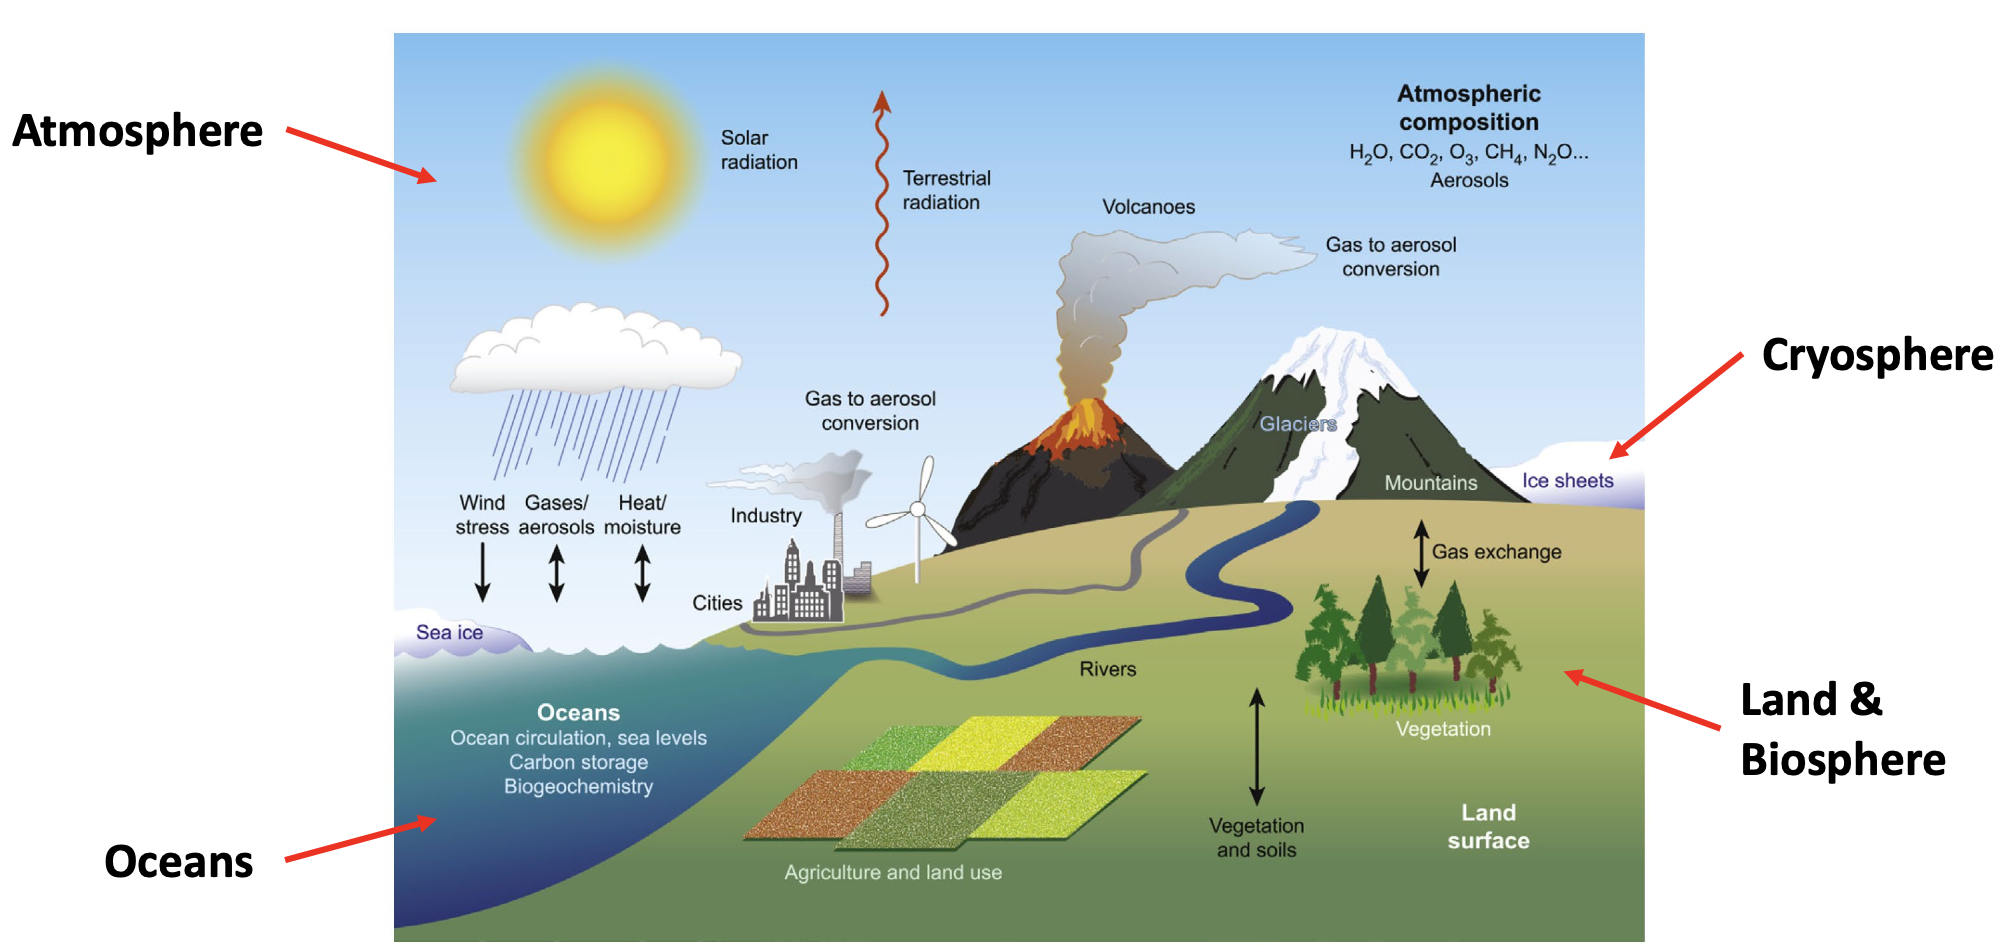
\includegraphics[width=1\linewidth]{CS//img/Components_Climate_System.png}
\end{figure}
The climate system consists of five main components:
\begin{itemize}
    \item \textbf{Atmosphere} – The gaseous layer surrounding Earth.
    \item \textbf{Oceans} – Regulate heat and carbon exchange.
    \item \textbf{Cryosphere} – Ice sheets, glaciers, and snow that impact global albedo.
    \item \textbf{Land \& Biosphere} – Vegetation and soil interactions with climate.
    \item \textbf{Anthropogenic Influence} – Human-induced changes to climate patterns.
\end{itemize}

\begin{figure}[H]
    \centering
    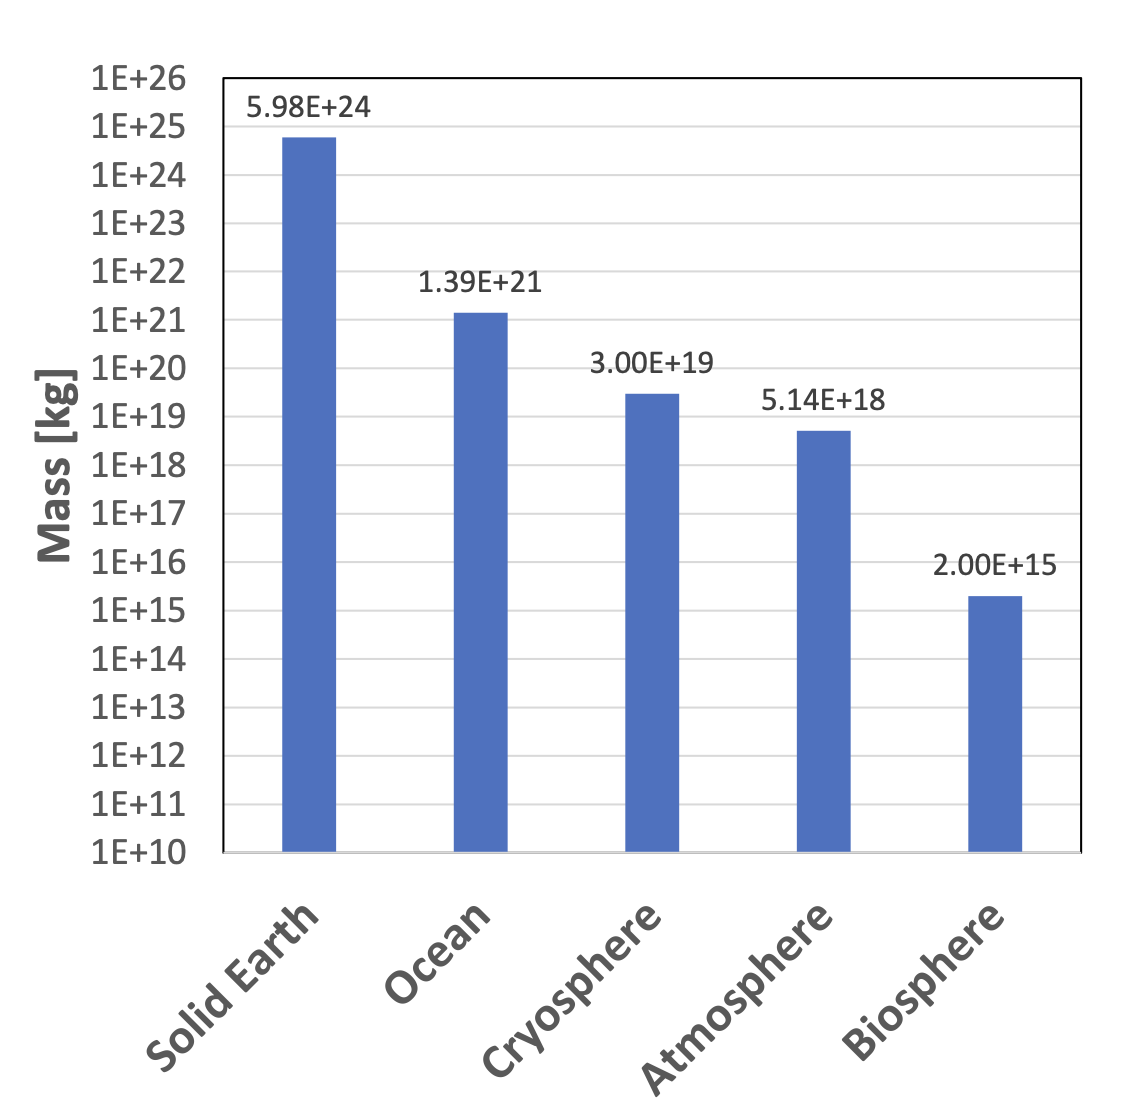
\includegraphics[width=0.8\linewidth]{CS//img/Abs_mass_components.png}
\end{figure}
\textbf{Logarithmic scale!!}\\
\subsection{Atmosphere and Energy Balance}
\begin{figure}[H]
    \centering
    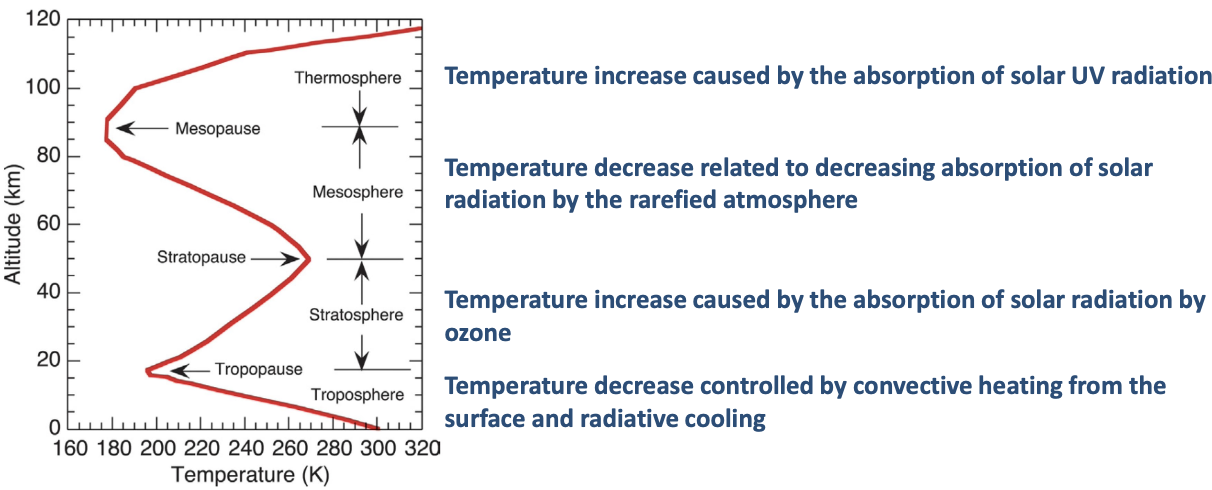
\includegraphics[width=\linewidth]{CS//img/Athmosphere.png}
\end{figure}
\begin{itemize}
    \item \textbf{Chemical Composition:}
    \begin{itemize}
        \item Major components: Nitrogen (N$_2$) and Oxygen (O$_2$)
        \item Important greenhouse gases: Water vapor, CO$_2$, Methane (CH$_4$)
    \end{itemize}
    \item \textbf{Vertical Structure of the Atmosphere:}
    \begin{itemize}
        \item Troposphere: Heated by convection and radiative cooling.
        \item Stratosphere: Temperature increases due to UV absorption by ozone.
    \end{itemize}
    \item \textbf{Global Energy Balance:} The climate system is driven by the balance between incoming solar radiation and outgoing infrared radiation.
    \item \textbf{Greenhouse Effect:} Contributes to warming by trapping heat.
\end{itemize}
\begin{figure}[H]
    \centering
    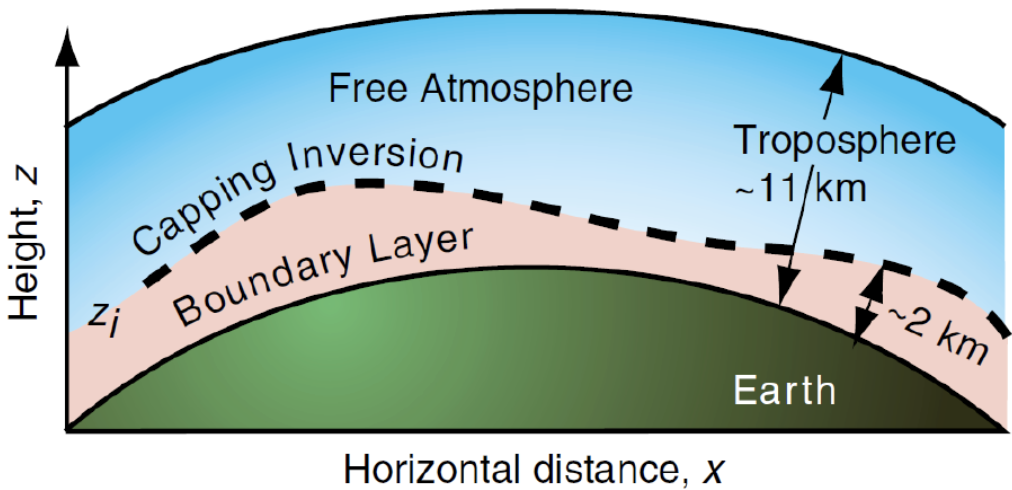
\includegraphics[width=0.5\linewidth]{CS//img/Planetary_layers.png}
\end{figure}
\begin{figure}[H]
    \centering
    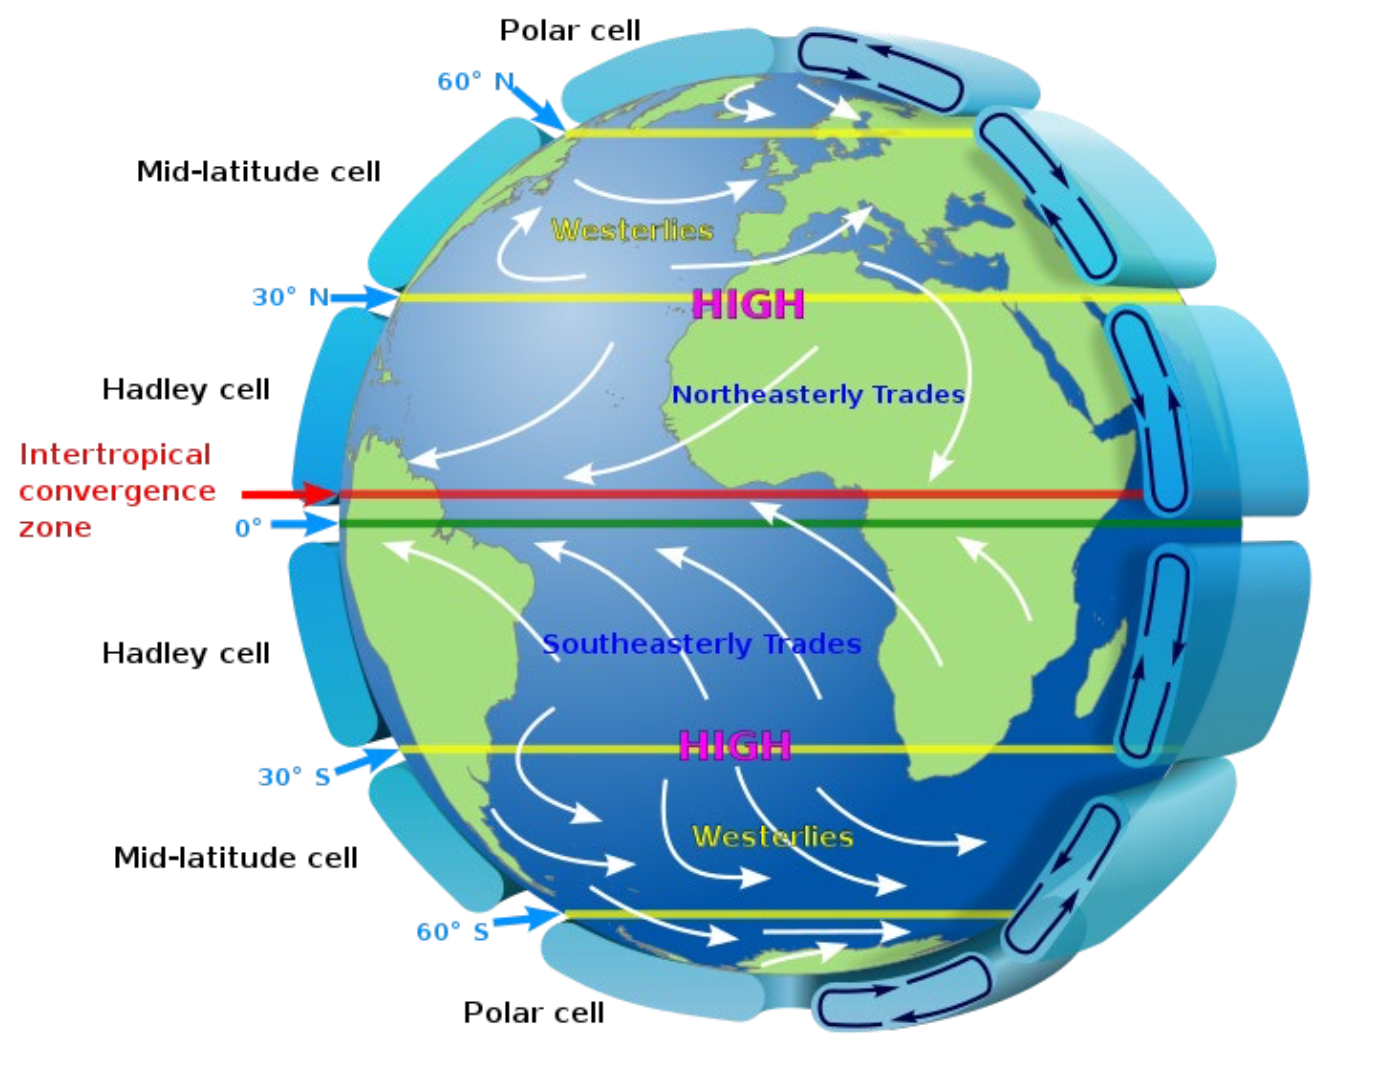
\includegraphics[width=1\linewidth]{CS//img/General_circulation_cells.png}
\end{figure}

\subsection{Oceans and Cryosphere}
\begin{itemize}
    \item \textbf{Thermohaline Circulation:} Deep ocean currents driven by differences in temperature and salinity.
    \item \textbf{Cryosphere Changes:} Rapid changes in ice sheets and glaciers affect sea level and energy balance.
\end{itemize}
\begin{figure}[H]
    \centering
    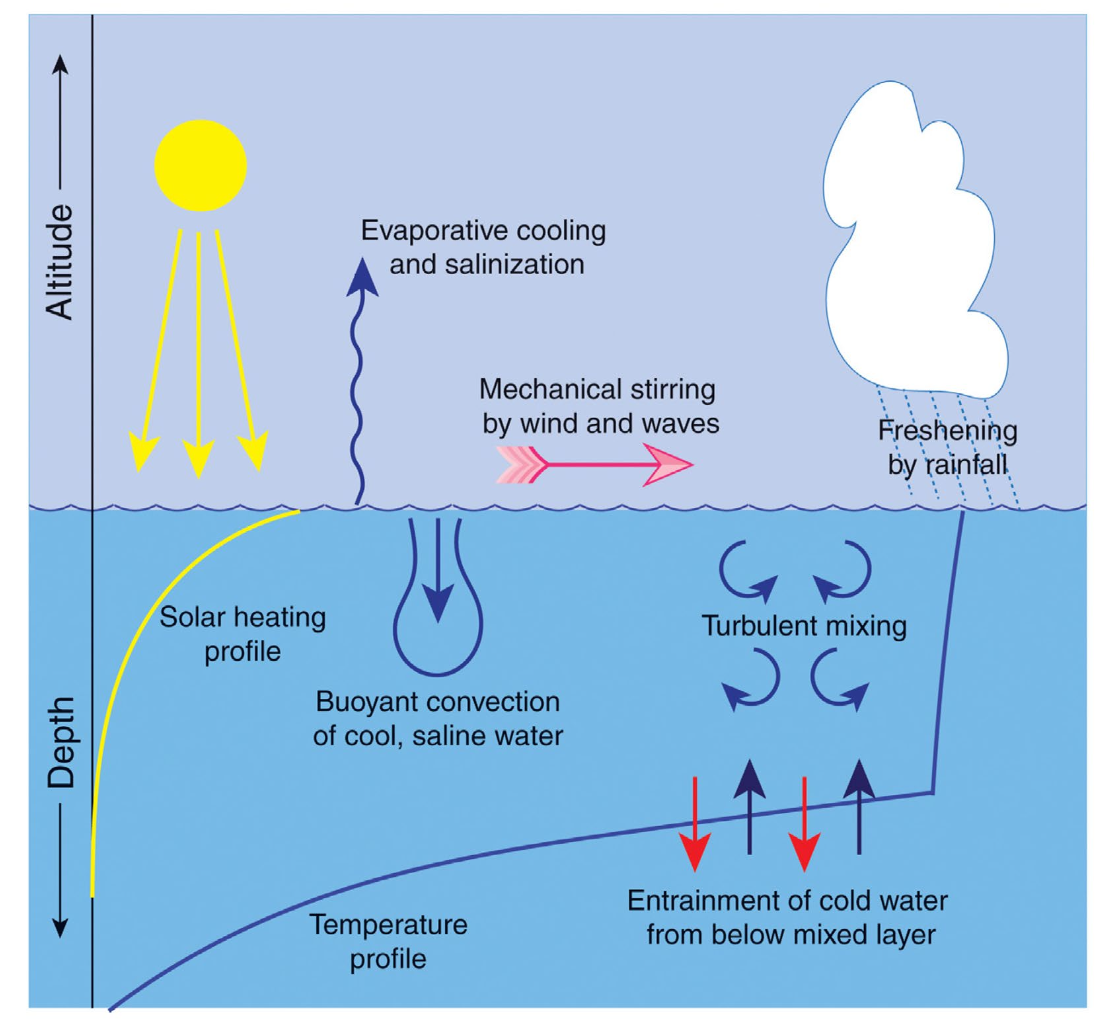
\includegraphics[width=0.8\linewidth]{CS//img/Athmosphere_Ocean_inteference.png}
\end{figure}
\subsection{Land, Biosphere, and the Carbon Cycle}
\begin{itemize}
    \item \textbf{Land Conditions Influence Climate:} Spatial and temporal variations affect temperature and precipitation.
    \item \textbf{Vegetation and the Carbon Cycle:}
    \begin{itemize}
        \item \textbf{Gross Primary Production (GPP):} Total carbon fixed by plants.
        \item \textbf{Net Primary Production (NPP):} GPP minus autotrophic respiration.
        \item \textbf{Net Biome Production (NBP):} Includes disturbances like wildfires and soil degradation.
    \end{itemize}
\end{itemize}

\subsection{Anthropogenic Climate Change}
\begin{itemize}
    \item \textbf{Global Temperature Increase:} +1.09$^{\circ}$C (2011-2020 compared to 1850-1900).
    \item \textbf{Rising CO$_2$ Concentrations:} Direct emissions from fossil fuels and land use changes.
    \item \textbf{Irreversible Impacts:} Some aspects, like Arctic ice loss, may be permanent on human timescales.
\end{itemize}

\begin{figure}[H]
    \centering
    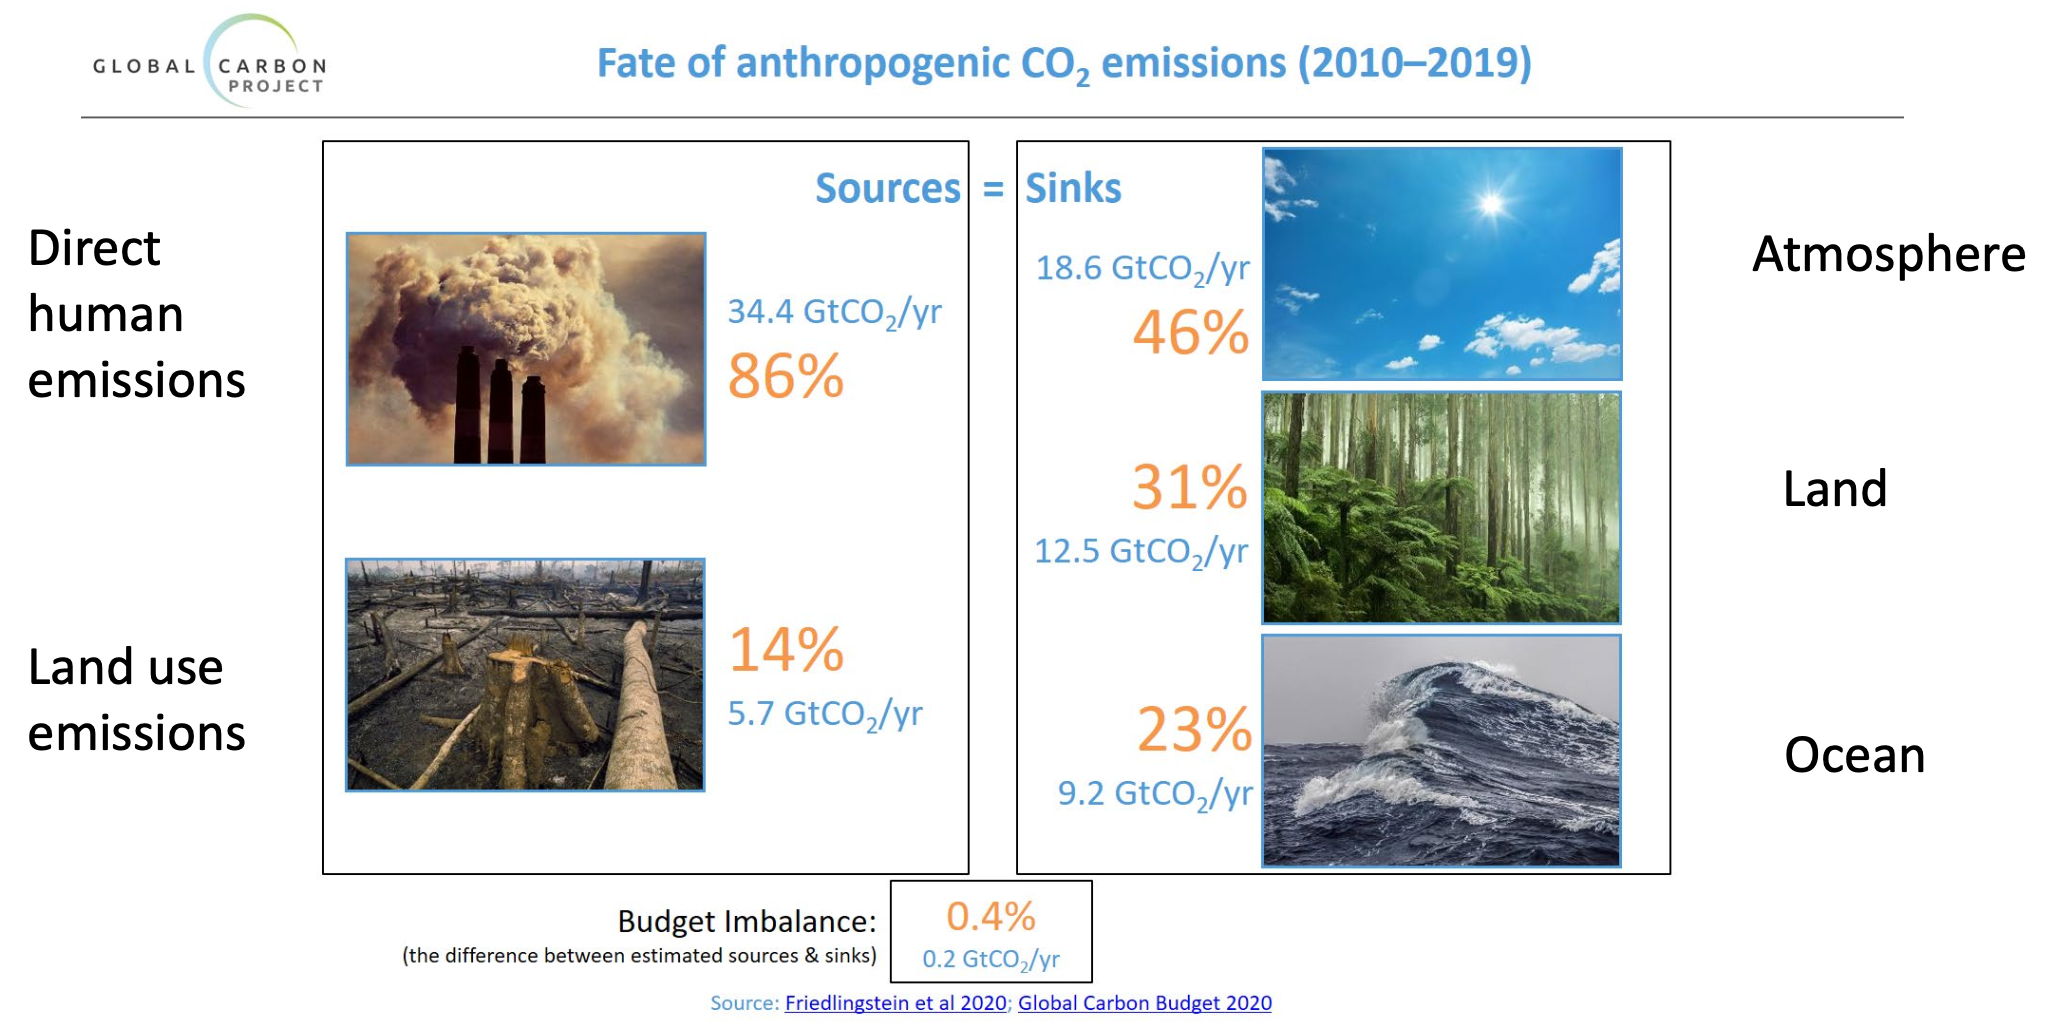
\includegraphics[width=1\linewidth]{CS//img/Global_Carbon_sink.png}
\end{figure}

\subsection{Global Climate Risks and Societal Implications}
\begin{itemize}
    \item \textbf{Impact on Key Sectors:}
    \begin{itemize}
        \item \textbf{Agriculture:} Growing seasons shift due to temperature changes.
        \item \textbf{Hydropower:} Variability in precipitation impacts energy production.
    \end{itemize}
    \item \textbf{Societal Challenges:}
    \begin{itemize}
        \item \textbf{Mitigation Efforts:} Reducing emissions.
        \item \textbf{Adaptation Strategies:} Preparing for changing climate conditions.
    \end{itemize}
\end{itemize}

\section{Atmospheric Radiative Transfer and the Global Energy Balance}
\noindent\textcolor{orange}{
Goal: Understand the Earth's energy budget, its role in the climate system, and how it is altered by anthropogenic influences.\\
Flow: Begins with fundamental radiation concepts, quantifies Earth's energy fluxes, assesses measurement techniques, and explores human impacts and implications.
}

\subsection{The Solar Source and Earth's Radiation Budget}

\begin{figure}[H]
        \centering
        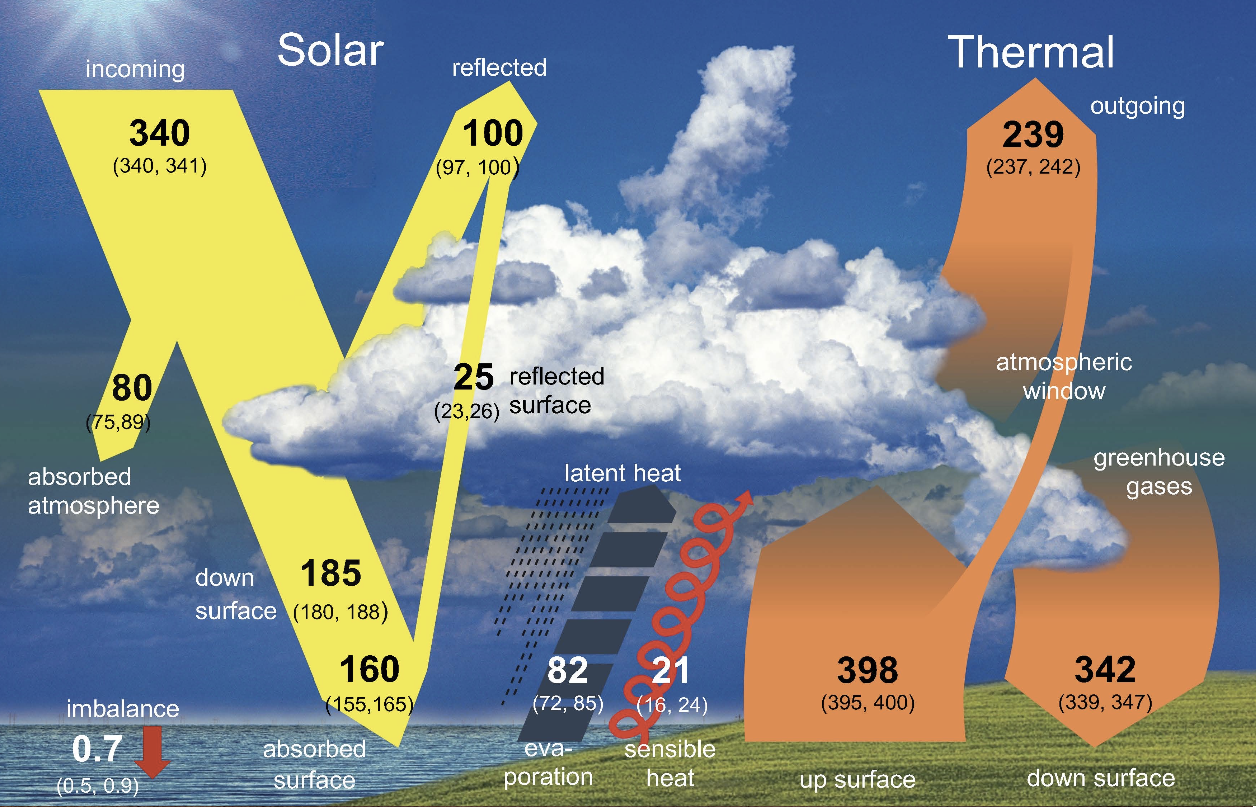
\includegraphics[width=0.75\linewidth]{CS//img/Basic_energy balance.png}
    \end{figure}
\begin{figure}[H]
    \centering
    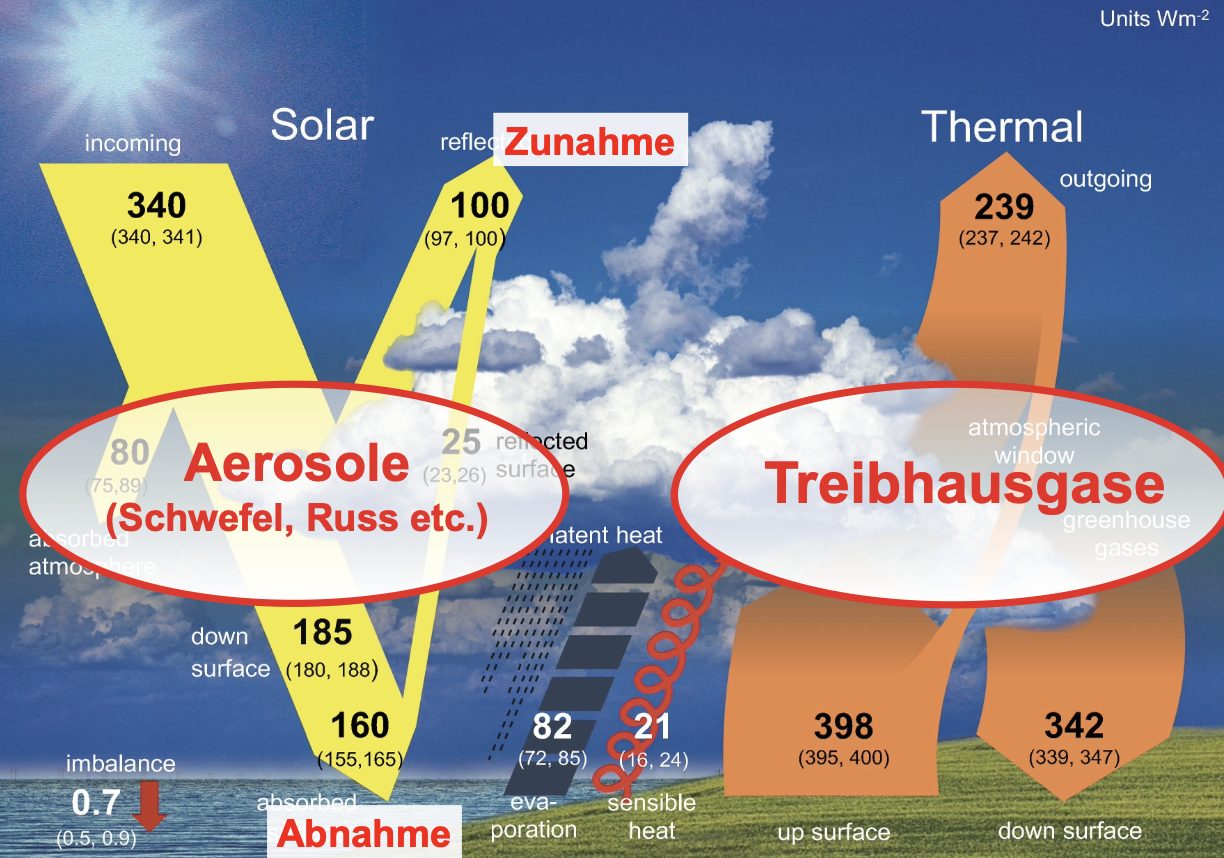
\includegraphics[width=.8\linewidth]{CS/img/Strahlungshaushalt.png}
\end{figure}
\[
\frac{\partial E_s}{\partial t} = G = R_s - LE - SH - \Delta F_{eo}
\]

\begin{itemize}
  \item $\frac{\partial E_s}{\partial t}$: Change in energy storage in surface soil and water
  \item $R_s$: Net radiative energy flux into the surface
  \item $LE$: Latent heat flux (evaporation)
  \item $SH$: Sensible heat flux (conduction/convection)
  \item $\Delta F_{eo}$: Horizontal subsurface energy flux (small on land)
\end{itemize}
\begin{itemize}
    \item The Sun provides $\sim$170 petawatts of energy to the Earth system—equivalent to 170 million nuclear power plants.
        \item $\sim$30\% of incoming solar radiation is reflected (albedo), while $\sim$70\% is absorbed by the atmosphere, clouds, and surface.
    \item The absorbed energy is re-emitted as thermal (longwave) radiation, creating a dynamic balance.
    \item The greenhouse effect arises from atmospheric gases absorbing outgoing longwave radiation and re-emitting it toward the surface.
\end{itemize}

\subsection{Top-of-Atmosphere and Surface Energy Balance}
\begin{itemize}
    \item Near the top of the atmosphere (TOA), absorbed solar radiation and outgoing longwave radiation are almost balanced.
    \item A small imbalance of \textbf{+0.7 Wm$^{-2}$} remains—this drives ongoing global warming.
    \item At the surface, the imbalance is more pronounced: \textbf{+104 Wm$^{-2}$} net radiation surplus, compensated by sensible and latent heat fluxes.
    \item The atmosphere exhibits a net radiative deficit of \textbf{-103 Wm$^{-2}$}, $\textbf{have to be compensated by sensible/latent heat}$
    \item Most of the energy imbalance is absorbed by the Ocean (91 $\%$)
\end{itemize}

\subsection{Solar Activity: Sunspots and Faculae}
\begin{itemize}
    \item The solar constant ($\sim$1361 Wm$^{-2}$, average amount of solar energy received per unit area at the top of Earth’s atmosphere, on a surface perpendicular to the Sun’s rays, at the mean Earth–Sun distance.) is not perfectly constant it varies slightly with solar activity cycles.
    \item \textbf{Sunspots} are darker, cooler regions on the Sun’s surface caused by magnetic activity. They reduce local solar output.
    \item However, sunspots are surrounded by \textbf{faculae}, which are brighter, hotter regions that increase solar output.
    \item During periods of high solar activity (solar maxima), the net effect of more faculae \textbf{overcompensates} for the darkening from sunspots.
    \item As a result, total solar irradiance (TSI) slightly \textbf{increases}—by about \textbf{0.1\%}—over the 11-year solar cycle.
    \item This small variation has limited effect on long-term climate trends compared to anthropogenic forcing.
\end{itemize}
\subsection{Spatial and Temporal Radiation Variability}

\begin{figure}[H]
    \centering
    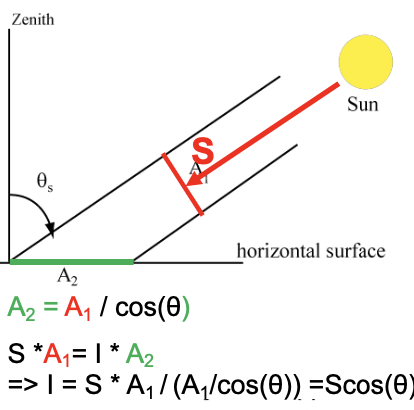
\includegraphics[width=0.2\linewidth]{CS//img/Isolation_at_specific_location.png}
\end{figure}
\begin{itemize}
    \item Radiation is strongly modulated by latitude, time of day, and season—governed by the solar zenith angle $\theta$.
    \item Instantaneous insolation (amount of solar radiation received at a specific location and time on a horizontal surface) is given by:
    \[
    I = S \cos(\theta)
    \]
    where $S$ is the solar constant ($\sim 1361\,\text{Wm}^{-2}$).
    \item The zenith angle $\theta$ depends on: \textit{(Zenith angle = angle between the direction of the Sun and the vertical; it is $0^\circ$ when the Sun is directly overhead = 90$^\circ$ horizon angle}
    \begin{itemize}
        \item \textbf{Time of day}, via the hour angle $H$, calculated as:
        \[
        H = \frac{\text{seconds till or from noon, 	( + for afternoon, – for morning)}}{86400} \cdot 360^\circ
        \]
        \item \textbf{Latitude} $\phi$ of the location.
        \item \textbf{Season}, represented by the solar declination angle $\delta$, which varies between $\pm 23.45^\circ$ throughout the year.
    \end{itemize}
    \item These three dependencies are combined in the full formula for the zenith angle:
    \[
    \cos \theta = \cos H \cos \phi \cos \delta + \sin \phi \sin \delta
    \]
    \begin{itemize}
        \item $\cos H$: controls the time of day
        \item $\phi$: represents the latitude, in degrees
        \item $\delta$: encodes the day of the year / season, $\delta \approx -23.45^\circ \cdot \cos\left( \frac{360}{365} \cdot (N + 10)^\circ \right)$
    \end{itemize}
\end{itemize}

\begin{figure}[H]
    \centering
    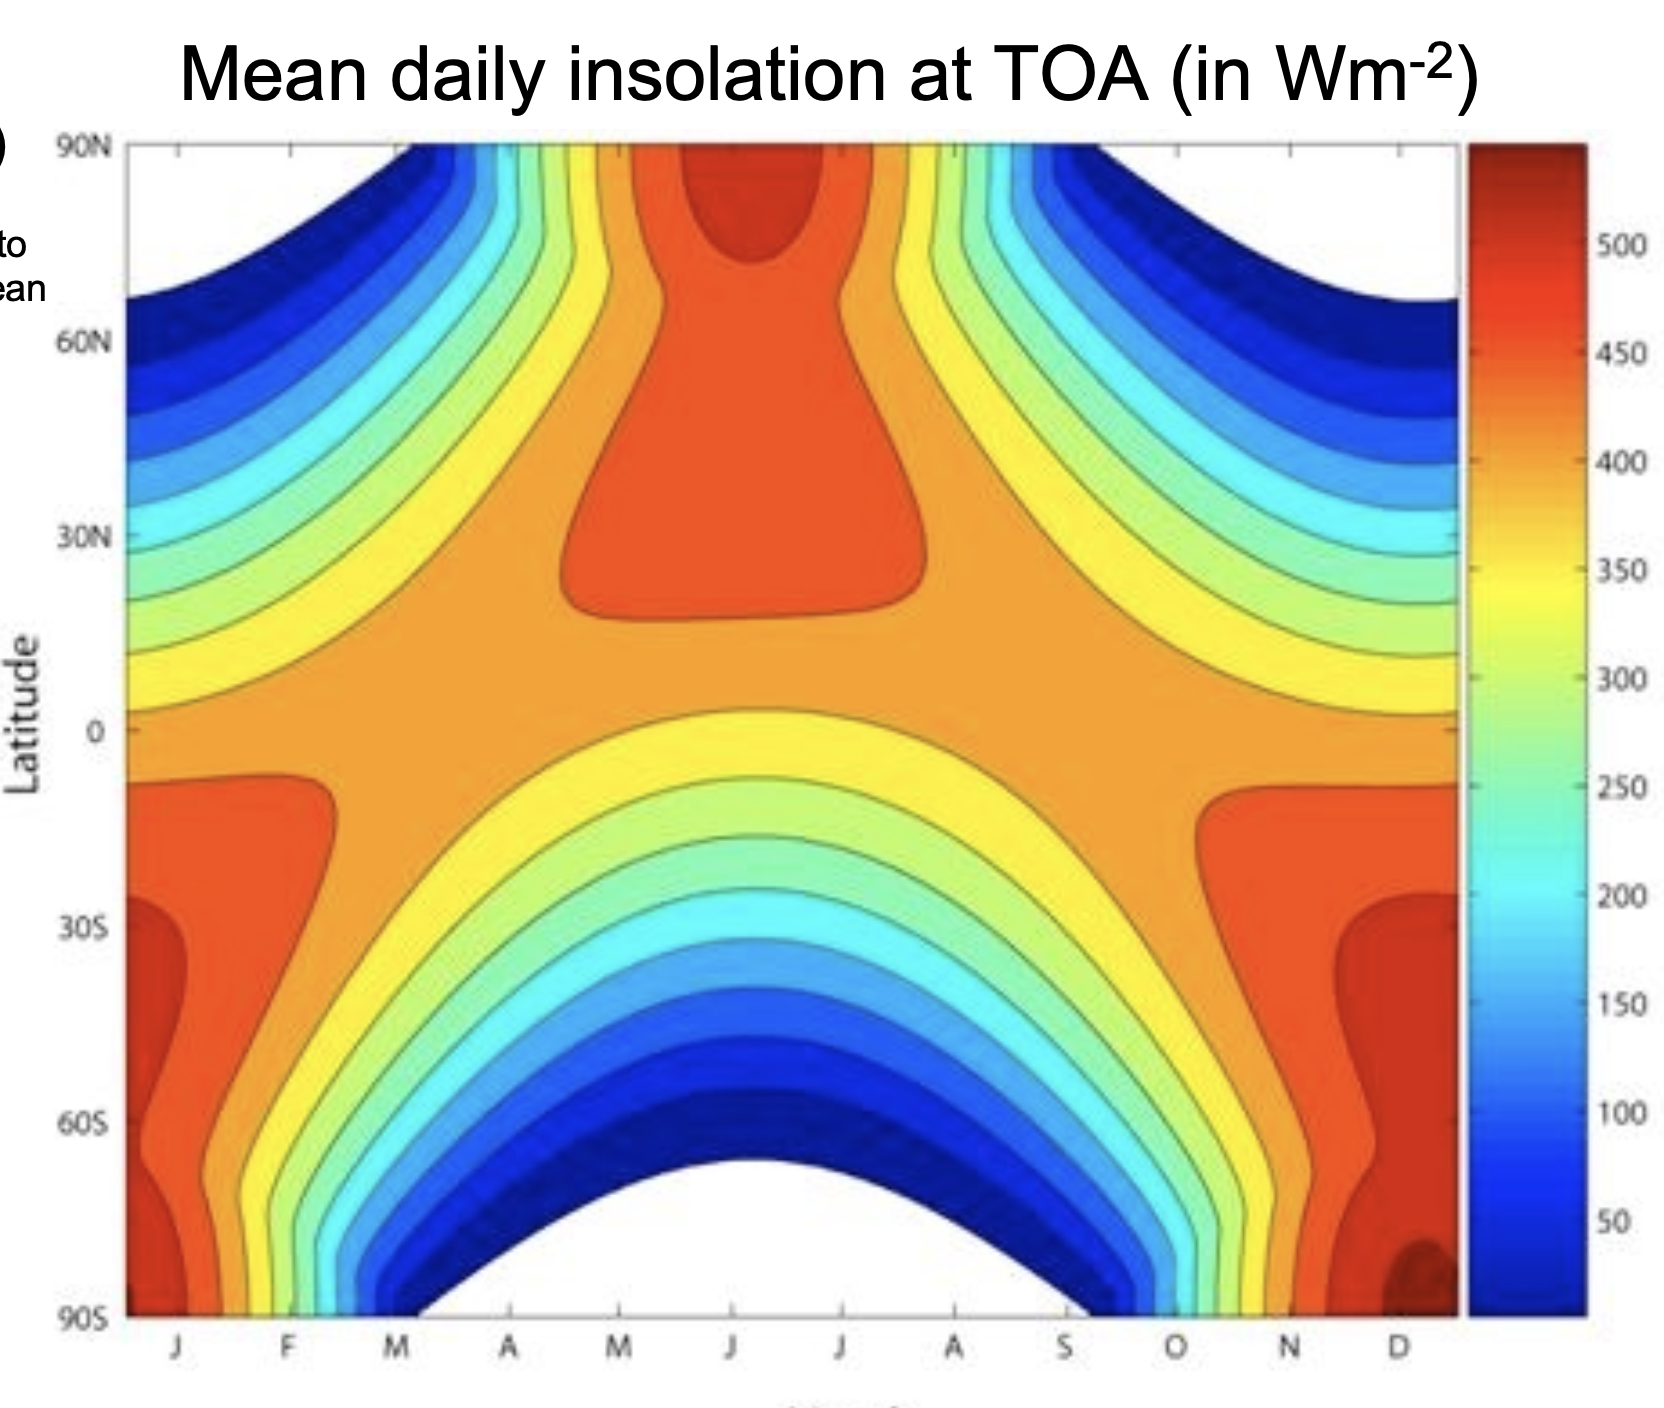
\includegraphics[width=0.5\linewidth]{CS//img/Mean_daily_isolation.58.png}
\end{figure}
\subsection{Atmospheric Radiative Transfer}
\begin{figure}[H]
    \centering
    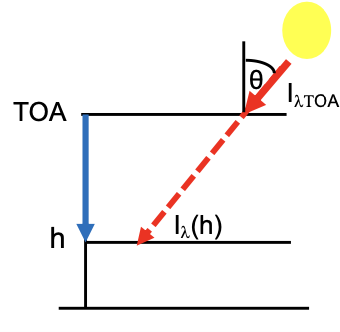
\includegraphics[width=0.2\linewidth]{CS//img/Attenuation.png}
\end{figure}
\begin{itemize}
    \item Insolation decreases with atmospheric depth and wavelength due to scattering and absorption:
    \[
    I_\lambda(h) = I_{\lambda,\mathrm{TOA}} e^{-\tau_\lambda m}
    \]
    \item $I_{\lambda,\mathrm{TOA}}$: Insolation at TOA
    \item $k_\lambda = k_{\lambda,abs}+k_{\lambda,scatt}$: Extinction coefficient, wavelength dependent with $k_{\lambda,abs}$ absorption coefficient, $k_{\lambda,scatt}$ scattering coefficient
    \item m: optical mass $= \frac{1}{cos(\theta)}$
    \item Extinction is composed of wavelength-dependent absorption ($k_{\lambda,\mathrm{abs}}$) and scattering ($k_{\lambda,\mathrm{scatt}}$).
\end{itemize}

\subsection{Anthropogenic Changes to Radiation Balance}
\begin{itemize}
    \item \textbf{Greenhouse gases (GHGs)}: Increase downward longwave radiation—observed trend: \textbf{+2 Wm$^{-2}$/decade}.
    \item \textbf{Aerosols}: Sulfates, soot, and organics scatter/absorb solar radiation. Effects:
    \begin{itemize}
        \item \textbf{Direct effect}: Reduces incoming shortwave radiation.
        \item \textbf{Indirect effect}: Alters cloud properties, enhancing cloud albedo and lifetime.
    \end{itemize}
    \item \textbf{Land-use changes}: Modify surface albedo, altering regional radiation budgets.
\end{itemize}

\subsection{Measuring Radiation Fluxes}
\begin{itemize}
    \item \textbf{Satellites} provide global coverage (e.g. ISCCP, CERES).
    \item \textbf{Ground stations (BSRN)} offer high-accuracy, long-term local observations.
    \item Uncertainties range from \textbf{±0.5 to ±5 Wm$^{-2}$}, depending on method and variable.
\end{itemize}

\subsection{Ocean Heat Uptake}
\begin{itemize}
    \item Oceans absorb \textbf{91\%} of the Earth’s excess energy since 1970.
    \item This is confirmed by Argo float temperature profiles in both upper and deep ocean layers.
    \item Ocean warming is the clearest signature of long-term Earth energy imbalance.
\end{itemize}

\subsection{Global Dimming and Brightening}
\begin{itemize}
    \item \textbf{1950s–1980s}: Increased aerosol emissions led to \textbf{global dimming}—a significant reduction in surface solar radiation due to both direct (scattering/absorption) and indirect (cloud-altering) aerosol effects.
    \item \textbf{Post-1980s}: Emission reductions in Europe and the USA resulted in \textbf{brightening}, revealing the full warming potential of greenhouse gases.
    \item Observations from Potsdam, China, and satellite data show $\sim$10\% variations in surface solar radiation during these periods.
    \item Although solar activity (sunspots and faculae) causes small variations in total solar irradiance ($\sim$0.1\%), these are \textbf{too small to explain} the observed dimming and brightening trends. Thus, \textbf{sunspots are not the cause of global dimming}.
    \item \textbf{Dimming and brightening trends are asymmetrical between hemispheres:}
    \begin{itemize}
        \item The \textbf{Northern Hemisphere (NH)} experienced strong dimming and later brightening due to heavy industrial aerosol emissions followed by air quality regulations.
        \item The \textbf{Southern Hemisphere (SH)} showed weaker trends, as fewer anthropogenic aerosols were emitted.
        \item This hemispheric difference is consistent with observed trends in temperature, radiation, and sulfur emissions.
    \end{itemize}
    \item Both direct and indirect aerosol effects (cloud albedo/cloud lifetime) reduce the amount of solar radiation reaching the ground
\end{itemize}

\subsection{Impacts on Climate and Society}
\begin{itemize}
    \item Dimming masked global warming, led to slowed glacier retreat and reduced rainfall (Swiss Glaciers area reduction: “Dimming phase“ 1973 - 1985: -1 $\%$, “Brightening phase“ 1985 – 2018: -33 $\%$.
    \item Brightening enhanced warming, hydrological intensification, and glacier melt.
    \item Aerosols affect PV efficiency: China could increase solar output by 11–15\% if pollution returned to 1960 levels (Sweerts et al. 2019).
\end{itemize}

\subsection{Photosynthesis and the Diffuse Radiation Effect}
\begin{itemize}
    \item \textbf{Diffuse radiation} from aerosols penetrates plant canopies better than direct sunlight.
    \item Leads to enhanced carbon uptake and increased plant productivity during dimming (Mercado et al. 2009).
\end{itemize}

\subsection{Conclusions}
\begin{itemize}
    \item The Earth's radiation balance is central to climate regulation.
    \item Human activities (GHGs, aerosols, land-use) significantly alter radiation transfer and energy fluxes.
    \item The radiation imbalance quantifies the magnitude of anthropogenic climate change.
    \item Monitoring surface and satellite radiation is essential for tracking climate dynamics and supporting mitigation strategies.
\end{itemize} 
\section{Climate Change \& IPCC Assessments}
\noindent\textcolor{orange}{
Goal: Present the current state of the climate crisis and the role of the IPCC.\\
Flow: Presents extreme events, explains IPCC's role and process, provides projections and mitigation strategies.
}

\subsection{Climate Crisis: Current Observations}
\begin{itemize}
    \item Climate crisis is evident with increasing extreme weather events worldwide.
    \item Record-breaking heatwaves, wildfires, and droughts have caused economic damages and loss of life.
    \item The global temperature has increased by approximately 1.1$^{\circ}$C from 1850-1900 to 2011-2020.
    \item Human activities, primarily CO$_2$ emissions from fossil fuels, are the dominant cause of observed warming.
    \item Atmospheric CO$_2$ concentrations have reached unprecedented levels, directly influencing global temperatures.
    \item Climate extremes, such as heavy precipitation, heatwaves, and droughts, have become more frequent and intense.
\end{itemize}

\subsection{The Role of the IPCC}
\begin{itemize}
    \item Established in 1988 by WMO and UNEP to assess climate change science.
    \item Provides scientific basis for policy decisions but remains policy-neutral.
    \item Reports undergo extensive review by scientists and governments to ensure objectivity.
    \item “Policy-relevant but not policy-prescriptive”: IPCC summarizes scientific consensus for decision-makers.
\end{itemize}
\begin{figure}[H]
    \centering
    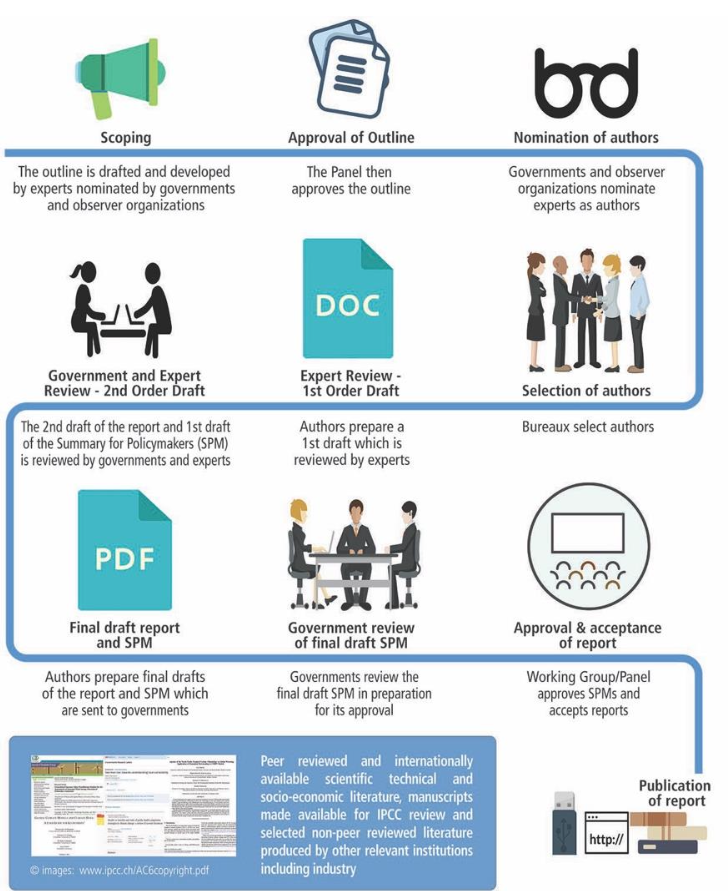
\includegraphics[width=0.8\linewidth]{Workings_of_IPCC.png}
\end{figure}
\subsection{Observed global warming}
\begin{figure}[H]
    \centering
    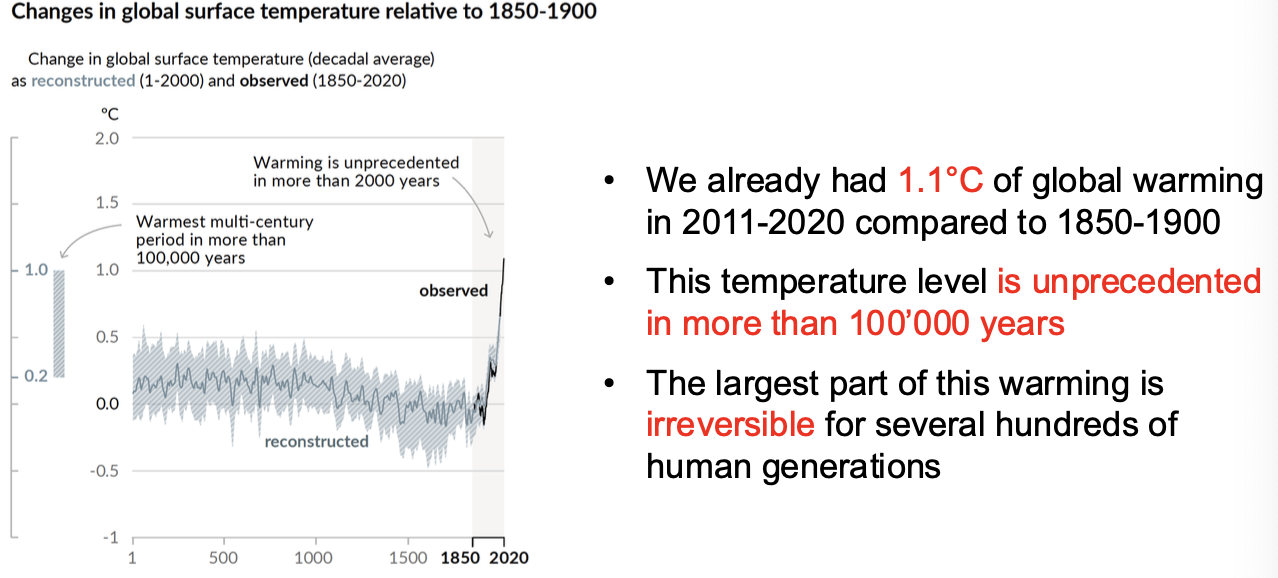
\includegraphics[width=1\linewidth]{CS//img/Observed_global_warming.png}
\end{figure}
\begin{figure}[H]
    \centering
    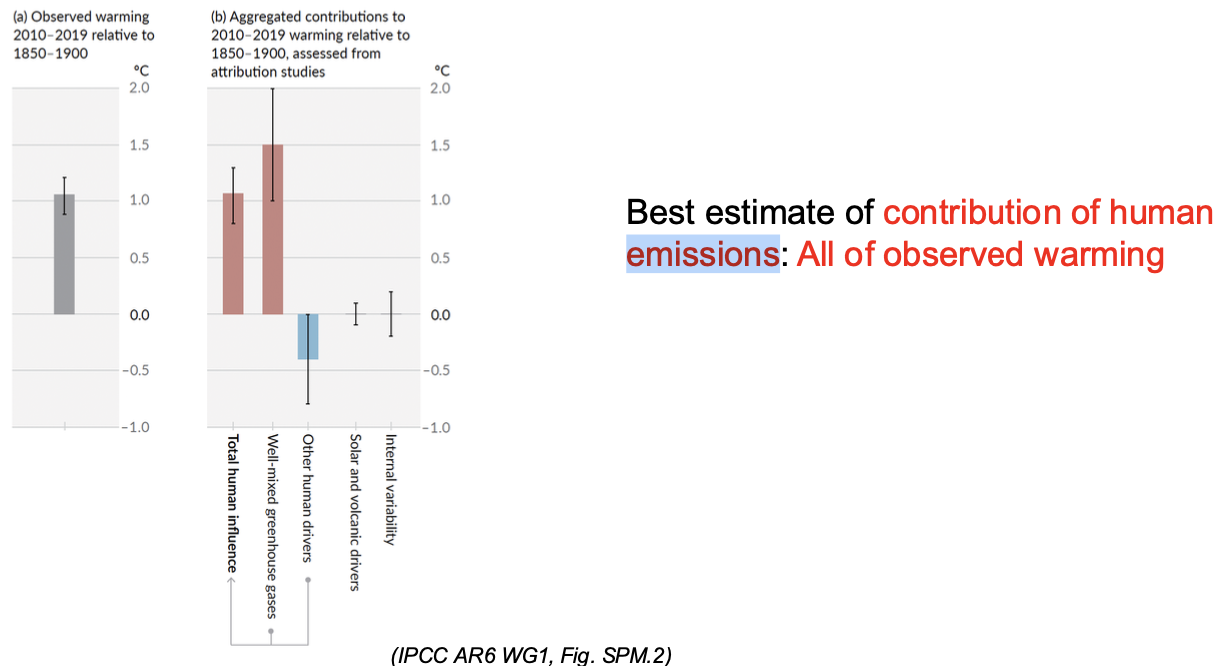
\includegraphics[width=1\linewidth]{CS//img/Observed_gw_2.png}
\end{figure}

\begin{figure}[H]
    \centering
    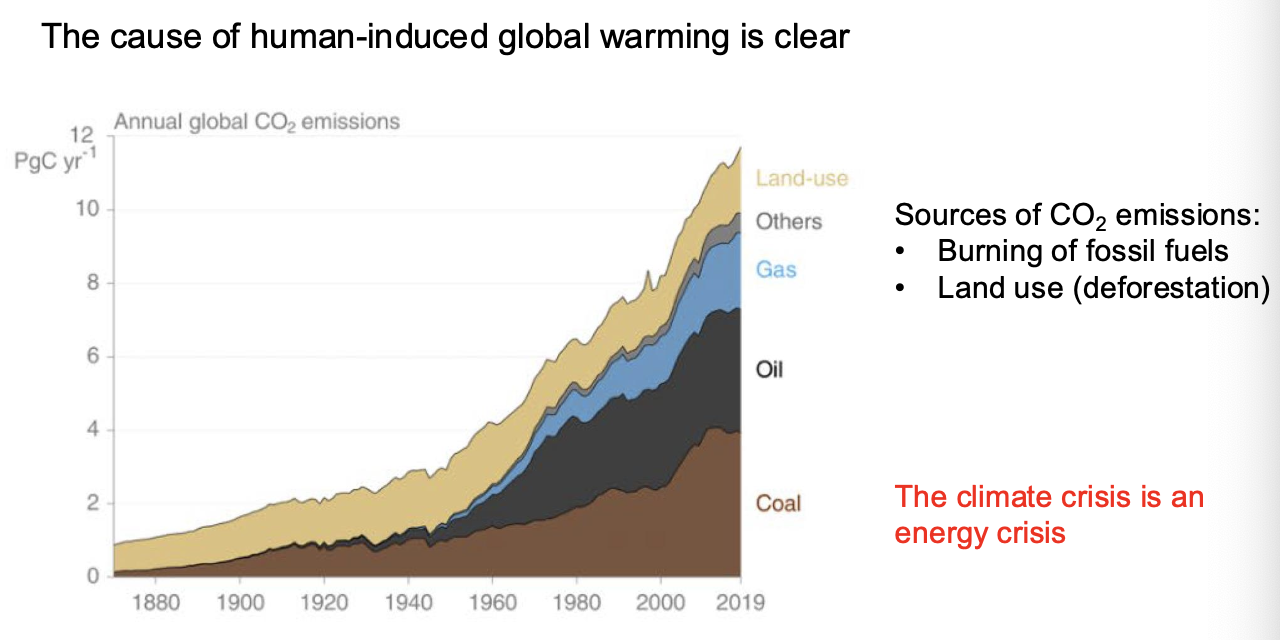
\includegraphics[width=0.9\linewidth]{CS//img/CO2_concentation.png}
\end{figure}

\begin{figure}[H]
    \centering
    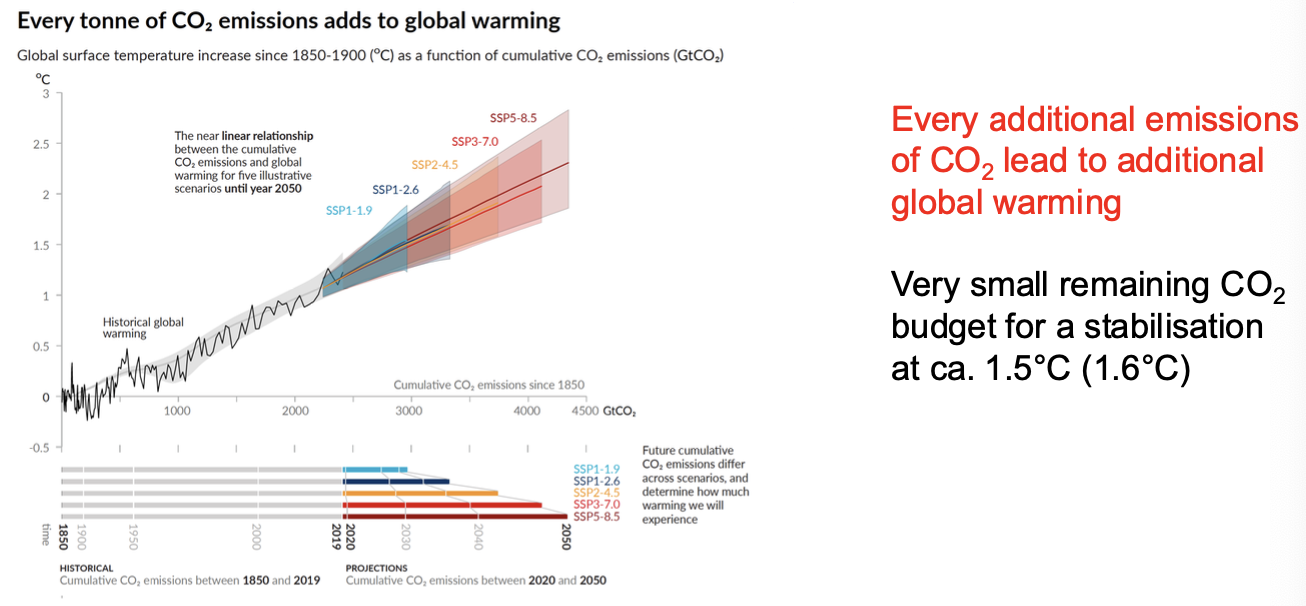
\includegraphics[width=0.9\linewidth]{CS//img/ton_of_Co2.png}
\end{figure} 
\begin{figure}[H]
    \centering
    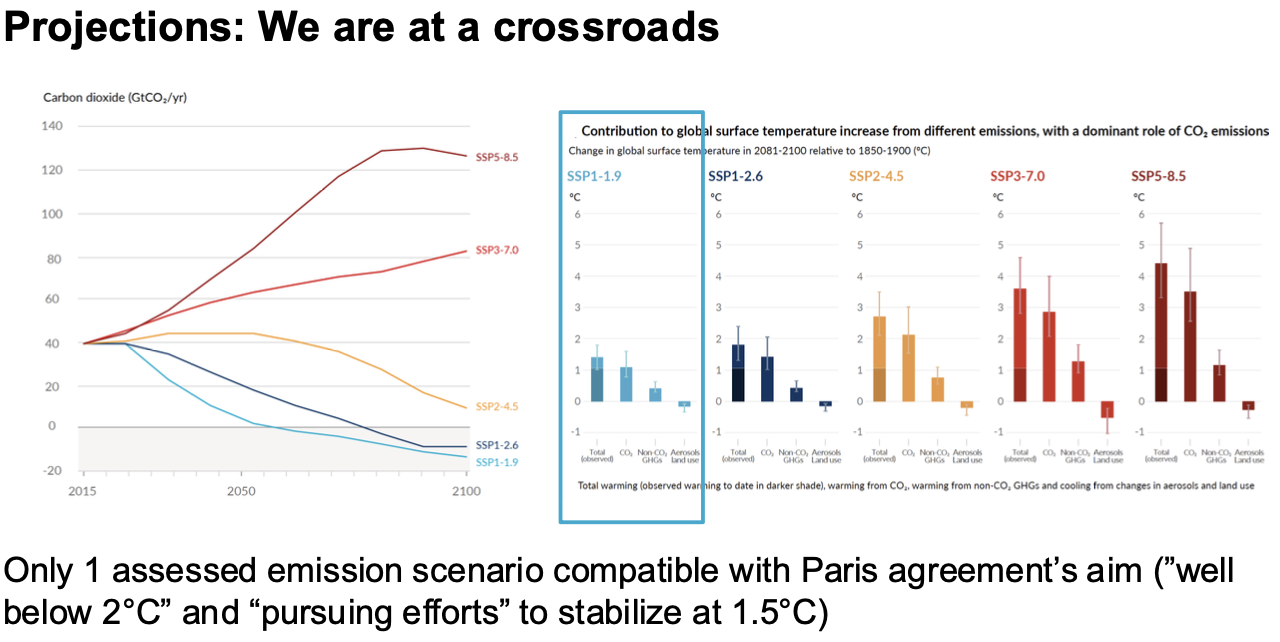
\includegraphics[width=0.9\linewidth]{CS//img/projections_crossroad.png}
\end{figure}







\subsection{Future Emission Scenarios}
\begin{figure}[H]
    \centering
    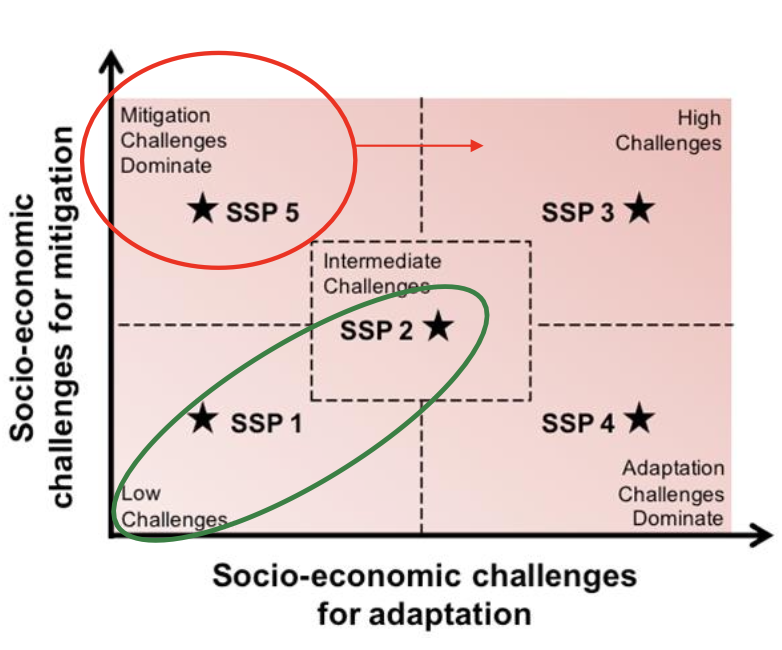
\includegraphics[width=0.6\linewidth]{CS//img/Scenarios_IPCC.png}
\end{figure}

\begin{figure}[H]
    \centering
    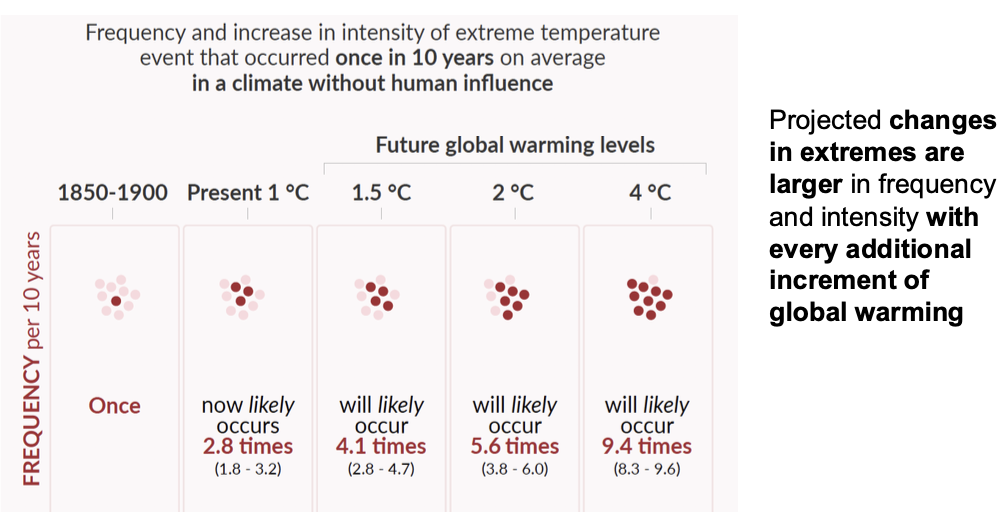
\includegraphics[width=1\linewidth]{CS//img/changes_in_extremes.png}
\end{figure}
\begin{itemize}
    \item IPCC assesses different socio-economic pathways (SSP scenarios) to project future warming.
    \item Only aggressive emissions reductions (SSP1) can keep global warming below 2$^{\circ}$C.
    \item The Coupled Model Intercomparison Project (CMIP) enables coordinated climate model simulations.
\end{itemize}

\subsection{Health and Economic Implications}
\begin{figure}[H]
    \centering
    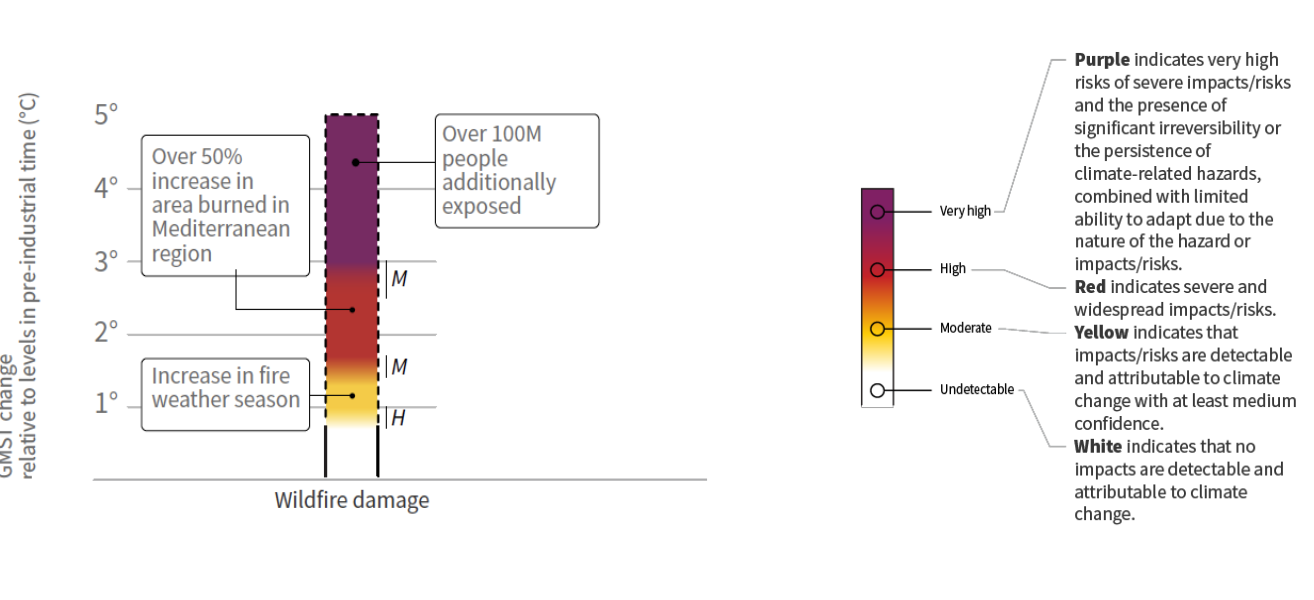
\includegraphics[width=1\linewidth]{CS//img/IPCC_IMPLICATIONS.png}
    \caption{Enter Caption}
    \label{fig:enter-label}
\end{figure}
\begin{itemize}
    \item Climate change already affects human health, with increased heat-related mortality.
    \item Economic impacts include damage to infrastructure, agriculture, and rising costs of climate adaptation.
    \item Fossil fuel phase-out improves air quality, benefiting human health and reducing healthcare costs.
\end{itemize}
\subsection{Scenarios for stabilization at $\approx$1.5°C}
\begin{itemize}
    \item Immediate reduction of CO2 emissions on global scale (until 2030: $50\%$ of 2010)
    \item Net-zero CO2 emissions at the latest in 2040 ($66\%$ probability) – 2050 ($50\%$ probability)
    \item “Negative emissions” after reaching net-zero CO2: At most $10\%$ of present- day emissions
\end{itemize}

\subsection{Pathway to Net-Zero Emissions}
\begin{itemize}
    \item “Zero” is more important than ”net”,is primarily about reducing CO2 emissions and the consumption of fossil fuels
    \item Hot do you reach net-zero?: No more use of fossil fuels (coal, oil, gas) ($90\%$ reduction of current CO2 emissions), $10\%$ compensation of CO2 emissions
    \item Transitioning to renewable energy, improving energy efficiency, and reforestation are key strategies.
    \item Net-zero means 90\% emissions reduction and only minimal negative emissions (e.g., afforestation).
\end{itemize}

\section{Fire and Ice: Past Climate Changes and Their Lessons for the Modern Climate Problem}
\noindent\textcolor{orange}{
Goal: Explore how past climate shifts from volcanic eruptions, monsoons, and orbital cycles inform present understanding.
Flow: From volcanic impacts and societal collapses to hydrological insights like aquifers and sea level rise.
}

\subsection{Volcanic Eruptions as Climate Influencers}
\begin{itemize}
\item Only explosive volcanic eruptions with viscous magma eject sulfur dioxide ($SO_2$) into the stratosphere, where it forms sulfate aerosols that reflect sunlight and increase planetary albedo, inducing global cooling.
\item Eruption location matters: Tropical eruptions are more effective in altering global climate because their aerosols spread to both hemispheres via stratospheric circulation.
\item The cooling impact depends on factors like aerosol optical depth, latitude, season, and feedback mechanisms such as increased sea ice cover and altered polar vortex dynamics.
\end{itemize}

\begin{figure}[H]
    \centering
    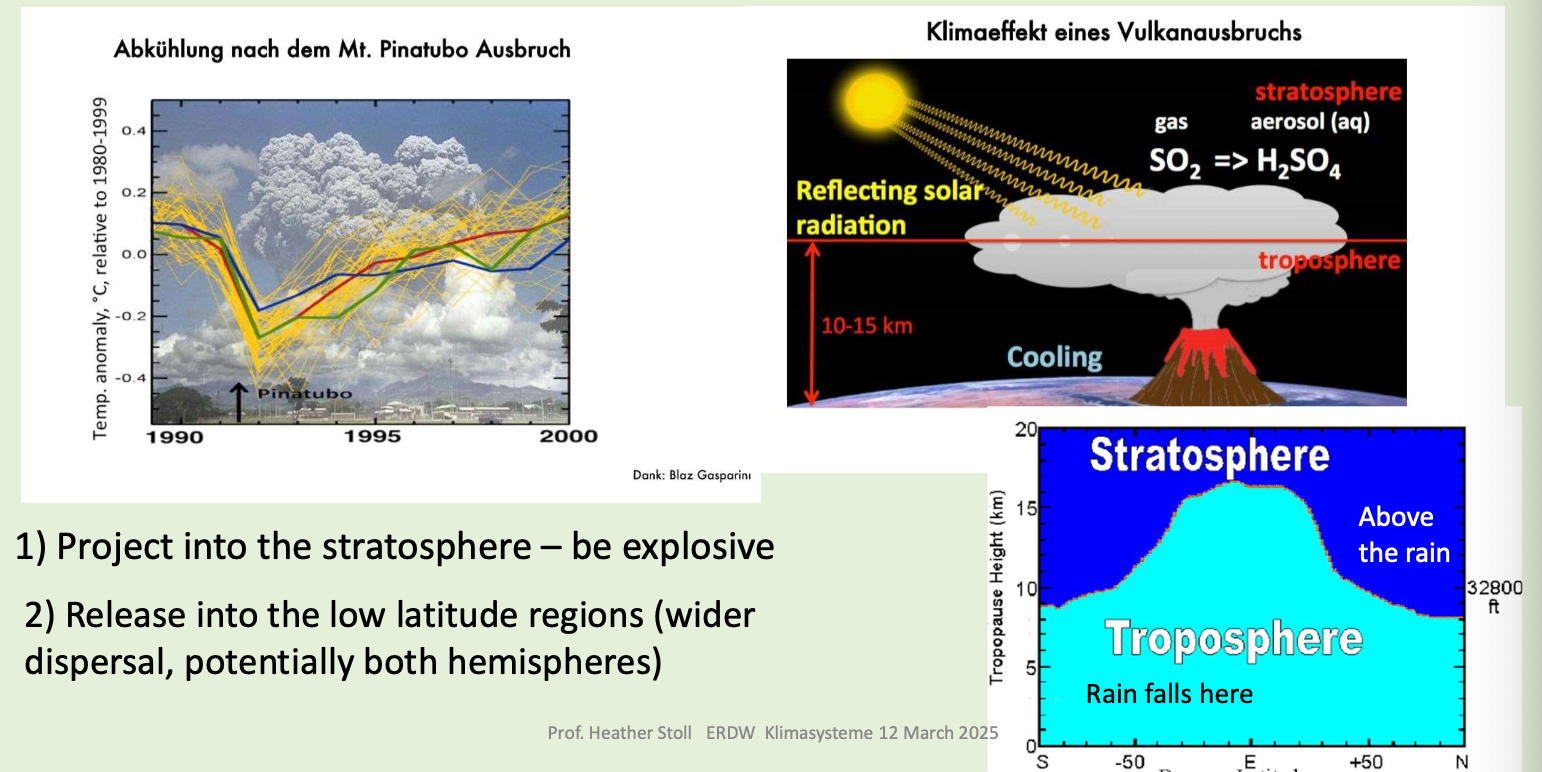
\includegraphics[width=1\linewidth]{CS//img/Vulcano_impact.png}
\end{figure}


\begin{figure}[H]
    \centering
    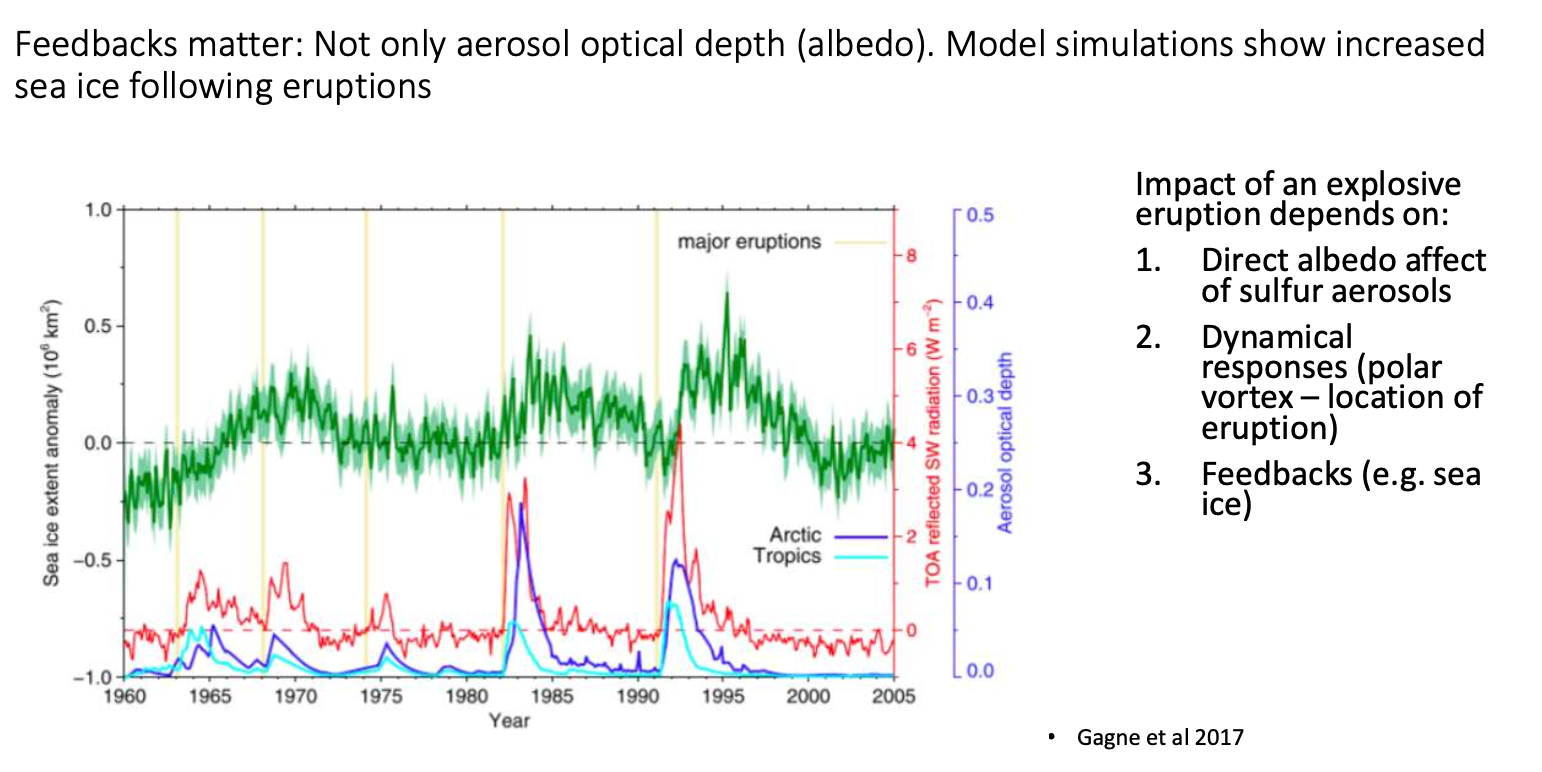
\includegraphics[width=1\linewidth]{CS//img/Vulcano_feedback.png}
\end{figure}
\subsection{Historical Examples of Volcanic Cooling}
\textbf{Sulfur from large volcanic eruptions can be detected in ice cores in Greenland and Antarctica (even if specific volcano is not known), Detection in both ice cores indicates a tropical eruption with global aerosol distribution}
\begin{itemize}
\item \textbf{Mt. Tambora (1816)}: One of the most powerful eruptions in the past 1500 years. Led to the “\textit{Year Without a Summer}” (1816), with crop failures, famines, and disease outbreaks in Europe and North America. Detected in both Greenland and Antarctic ice cores.
\item \textbf{Mt. Pinatubo (1991)}: Its sulfate aerosol veil caused ~0.5°C global cooling for 1–2 years. Used as a modern analogue in climate modeling.
\item \textbf{Late Antiquity Eruptions (536–540 AD)}:
\begin{itemize}
\item 536 AD: An extratropical eruption (likely NH) deposited sulfate in Greenland ice cores.
\item 541 AD: A second, larger tropical eruption, found in both Greenland and Antarctica ice cores, led to global aerosol dispersal.
\item These consecutive eruptions triggered a decade of cooling, known as the \textbf{Late Antique Little Ice Age (LALIA)}.
\item Crop failures, famines, and malnutrition weakened populations across the Byzantine Empire and Europe, creating ideal conditions for the outbreak of the \textbf{Justinianic Plague}.
\end{itemize}
\item Tree-ring reconstructions (e.g., from the Alps and Altai) confirm widespread temperature drops after major tropical eruptions.
\end{itemize}

\subsection{Water-The Nubian Aquifer}
\begin{itemize}
\item One of the largest fossil aquifers, containing \textasciitilde100,000 km³ of groundwater.
\item Its last major recharge occurred around 10,000 years ago during the Green Sahara period, when \textcolor{red}{increased Northern Hemisphere summer insolation intensified African monsoons}.
\item Future recharge is unlikely under current conditions—would require major orbital or climate shifts, which occur on multi-millennial timescales.
\end{itemize}

\subsection{Monsoon Variability and Insolation Changes}
\begin{itemize}
\item Seasonal ITCZ shifts drive monsoon dynamics; stronger summer insolation in the Northern Hemisphere historically intensified monsoons.
\item \textbf{Stalagmite records from China} reveal a strong monsoon response to past insolation cycles, supporting model predictions.
\item Kathmandu rainfall reconstructions suggest total annual precipitation was much higher 10,000 years ago than today.
\end{itemize}

\begin{figure}[H]
    \centering
    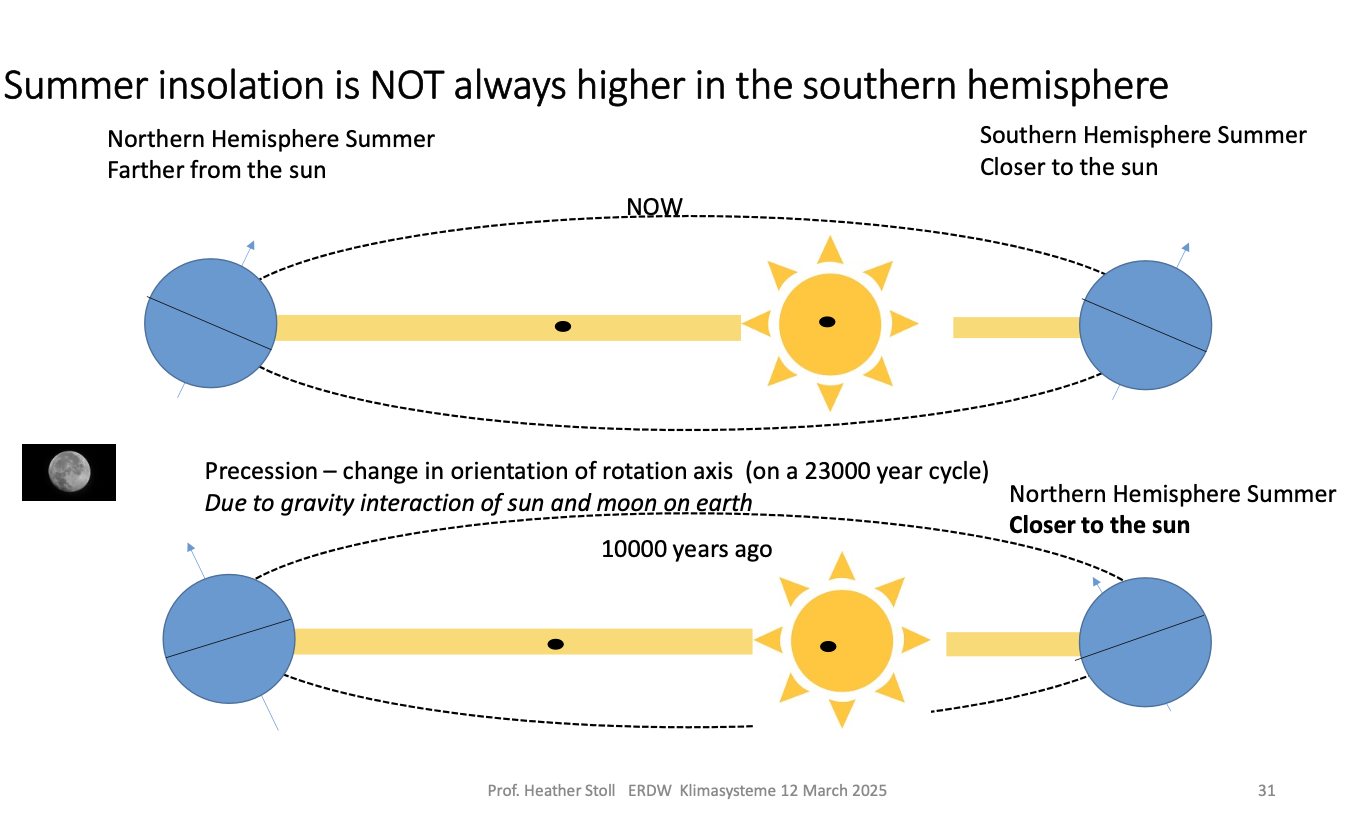
\includegraphics[width=1\linewidth]{CS//img/Summer_insolation.png}
\end{figure}
\subsection{Future Climate Implications}
\begin{itemize}
\item Anthropogenic forcing (GHGs, aerosols, land use change) influences monsoon systems—some regions may see stronger monsoons, others weaker.
\item \textbf{Erratic rainfall patterns} may increase, exacerbating droughts and floods.
\item Lessons from paleomonsoon systems help refine models of future hydrological cycle changes.
\end{itemize}


\subsection{Sea Level Rise in Past and Future}

\textbf{Question:} How fast can sea level rise?

\begin{itemize}
    \item The IPCC projects up to {0.8}{m} sea level rise by 2100 due to thermal expansion and glacier melt.
    \item In Earth's history, \textbf{Homo sapiens has experienced much faster sea level rise} — especially during deglaciations.
    \item Example: During the last deglaciation, rates reached \textbf{several meters per century}, due to rapid ice sheet collapses (e.g. \textit{ice saddle collapse}, \textit{marine ice sheet instability}).
\end{itemize}
\begin{figure}[H]
    \centering
    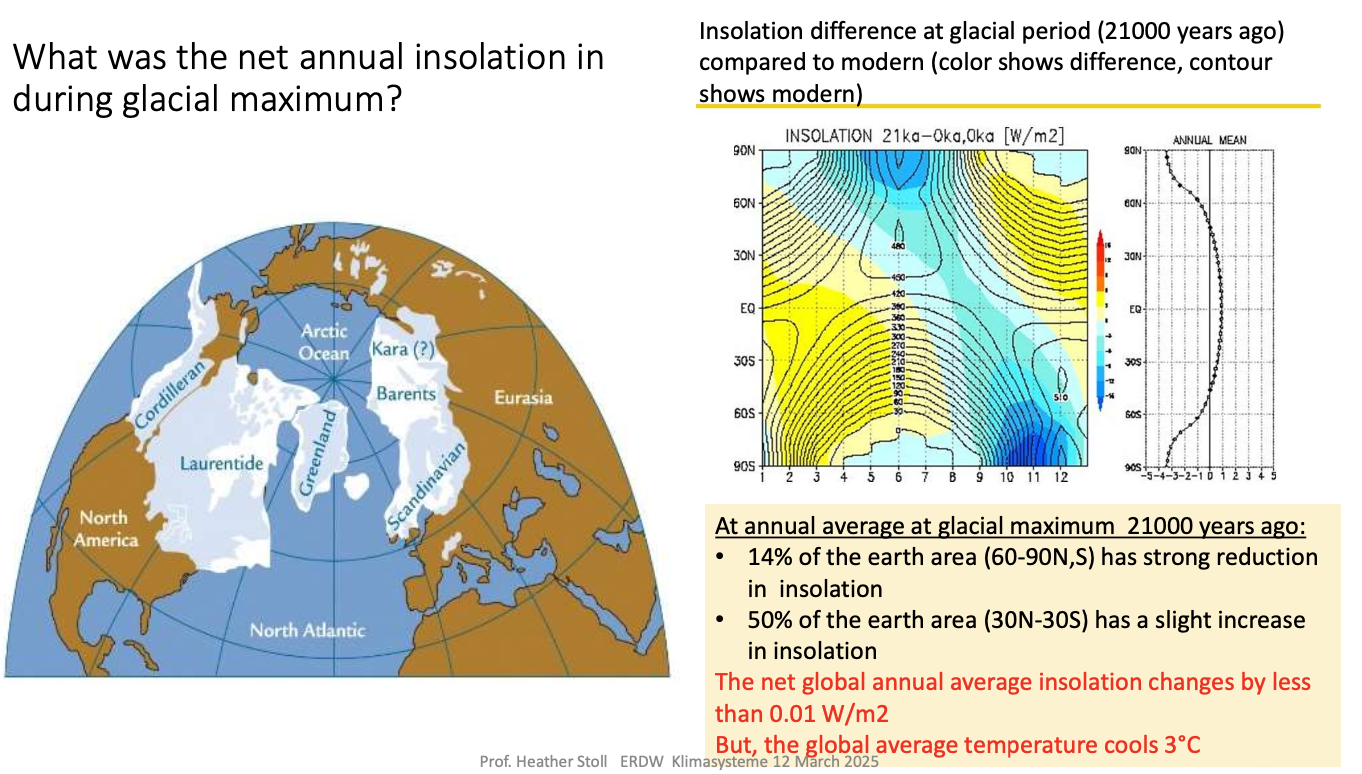
\includegraphics[width=0.5\linewidth]{CS/img/Ice_annual_insulation.png}

\end{figure}
\subsection{How can global temperature cool by 3°C with negligible change in global mean insolation?}

\textbf{Insight:} At the Last Glacial Maximum (21,000 years ago), global insolation changed by less than {0.01}{W/$m^2$}, yet Earth cooled by {3}{$^\circ$}.

\begin{itemize}
    \item This is explained by:
    \begin{itemize}
        \item \textbf{Regional and seasonal changes in insolation} — e.g. reduced summer insolation at high latitudes.
        \item \textbf{Feedbacks:} Ice-albedo feedback amplified small insolation shifts.
        \item \textbf{Greenhouse gas feedback:} Colder oceans absorbed more CO\textsubscript{2}, reducing the greenhouse effect.
    \end{itemize}
\end{itemize}

\subsection{What drives ice sheet growth?}

\textbf{Question:} Is it unusually low winter or summer insolation?

\begin{itemize}
    \item \textbf{Answer:} \textbf{Unusually low summer insolation} (especially at high northern latitudes) is key.
    \item Reason: Less summer melting allows snow to persist and build into ice sheets over time.
\end{itemize}

\subsection{What drives ice sheet retreat?}

\textbf{Question:} Is it unusually high winter or summer insolation?

\begin{itemize}
    \item \textbf{Answer:} \textbf{Unusually high summer insolation} leads to increased melting and retreat of ice sheets.
    \item Evidence from past interglacial periods shows this link clearly.
\end{itemize}

\subsection{Deglacial Melt and Ocean Circulation}

\begin{itemize}
    \item Rapid ice sheet melt releases freshwater into the North Atlantic.
    \item This can weaken the \textbf{Atlantic Meridional Overturning Circulation (AMOC)} within decades in climate models.
    \item Consequences include regional cooling in Europe despite global warming.
\end{itemize}

\subsection{Past vs Future}

\begin{itemize}
    \item Past meltwater pulses (e.g. from Laurentide Ice Sheet) likely caused AMOC slowdowns and abrupt climate events.
    \item The sensitivity of AMOC to freshwater forcing is still debated but supported by paleo climate evidence.
\end{itemize}

\section{Global Water Cycle}
\noindent\textcolor{orange}{
Goal: Analyze how water moves through the Earth system and how it's affected by climate change.\\
Flow: Goes from storage units and fluxes to regional water balance and finally to climate-driven changes in hydrology.
}
\subsection{The Role of Water in the Earth System}
\begin{itemize}
    \item Water is crucial for energy storage, atmospheric processes, and ecosystem functioning.
    \item Influences include the distribution of precipitation, evapotranspiration, and runoff.
    \item Water affects and is affected by radiation, temperature, and circulation patterns.
\end{itemize}

\subsection{Common Water Units}
\begin{itemize}
    \item \textbf{Mass [kg]} – Conserved quantity.
    \item \textbf{Volume [m$^3$]} – Depends on water density ($\rho \approx 1000$ kg/m$^3$).
    \item \textbf{Depth [mm]} – Volume per area, used for spatially distributed water.
\end{itemize}

\subsection{Global Water Storage and Distribution}
Total water on Earth(1 380 000 thousand km3) of this: Oceans, inland seas and saline lakes (97$\%$), Saline groundwater (less than $2\%$, Fresh water, only usable (less than $2\%$) \\
\begin{figure}[H]
    \centering
    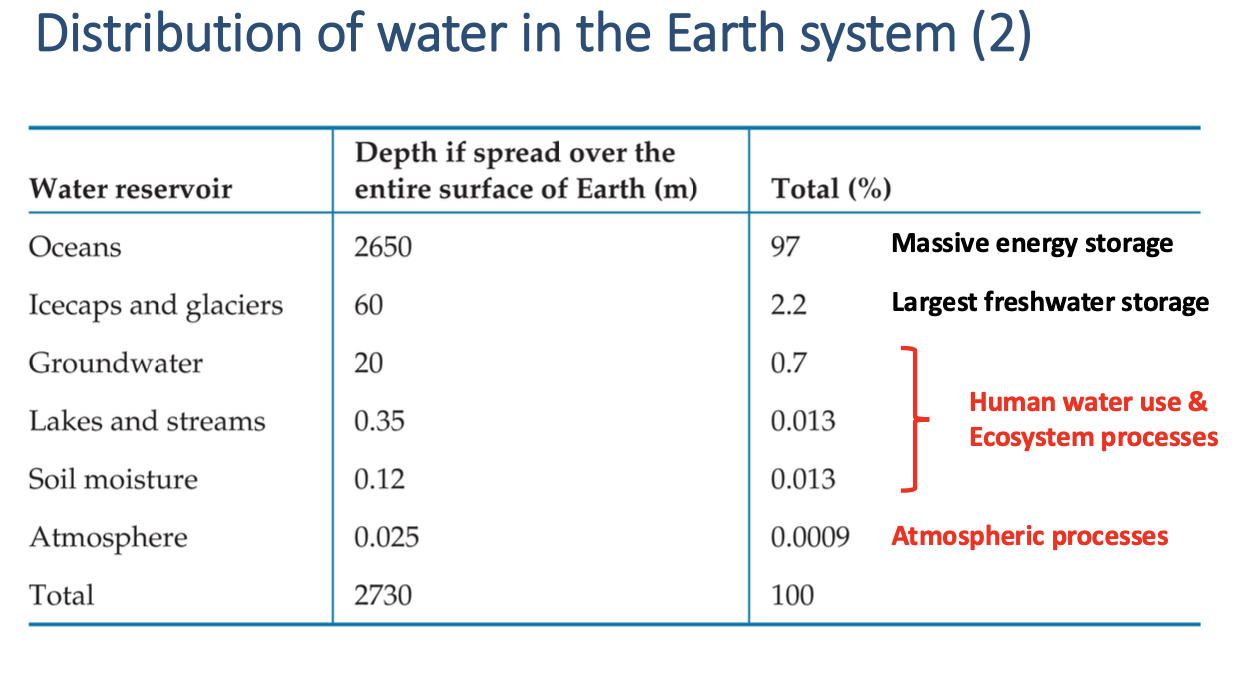
\includegraphics[width=\linewidth]{CS/img/Dist_water.png}
\end{figure}

\begin{figure}[H]
    \centering
    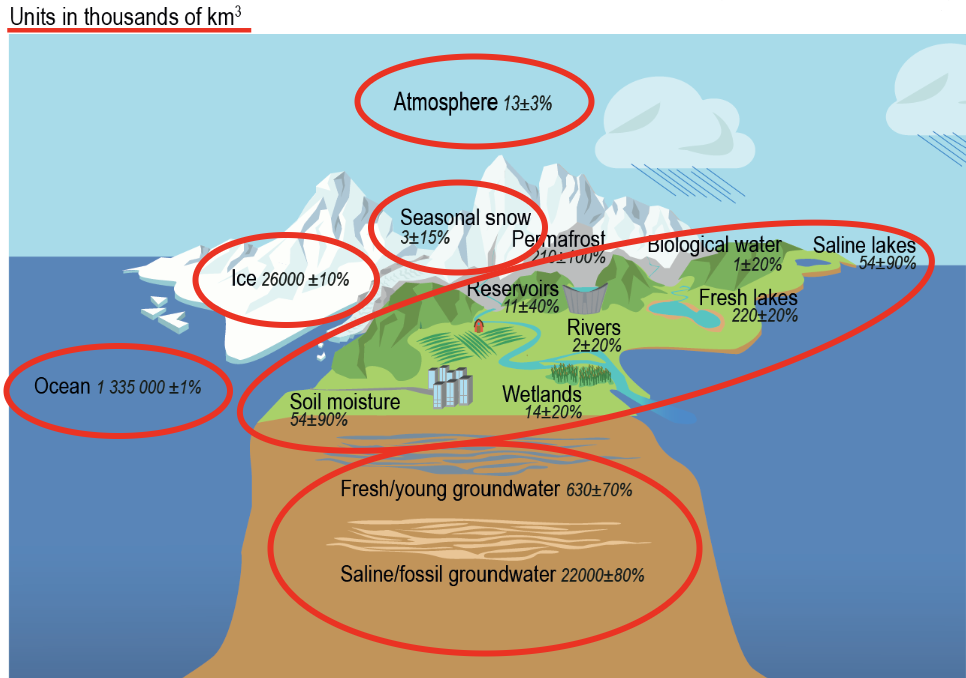
\includegraphics[width=\linewidth]{CS/img/global_water_storage.png}
\end{figure}
\subsection{Water Fluxes and Balances}
\begin{figure}[H]
    \centering
    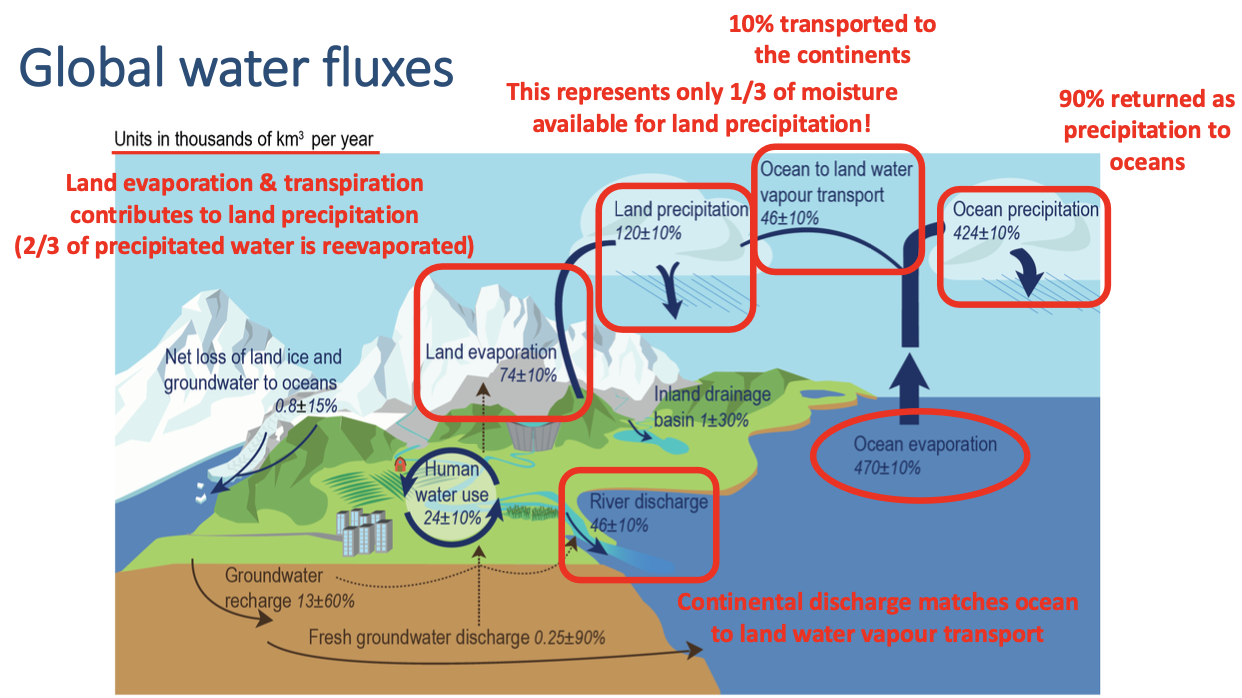
\includegraphics[width=1\linewidth]{CS//img/Water_flux.png}
\end{figure}

\begin{figure}[H]
    \centering
    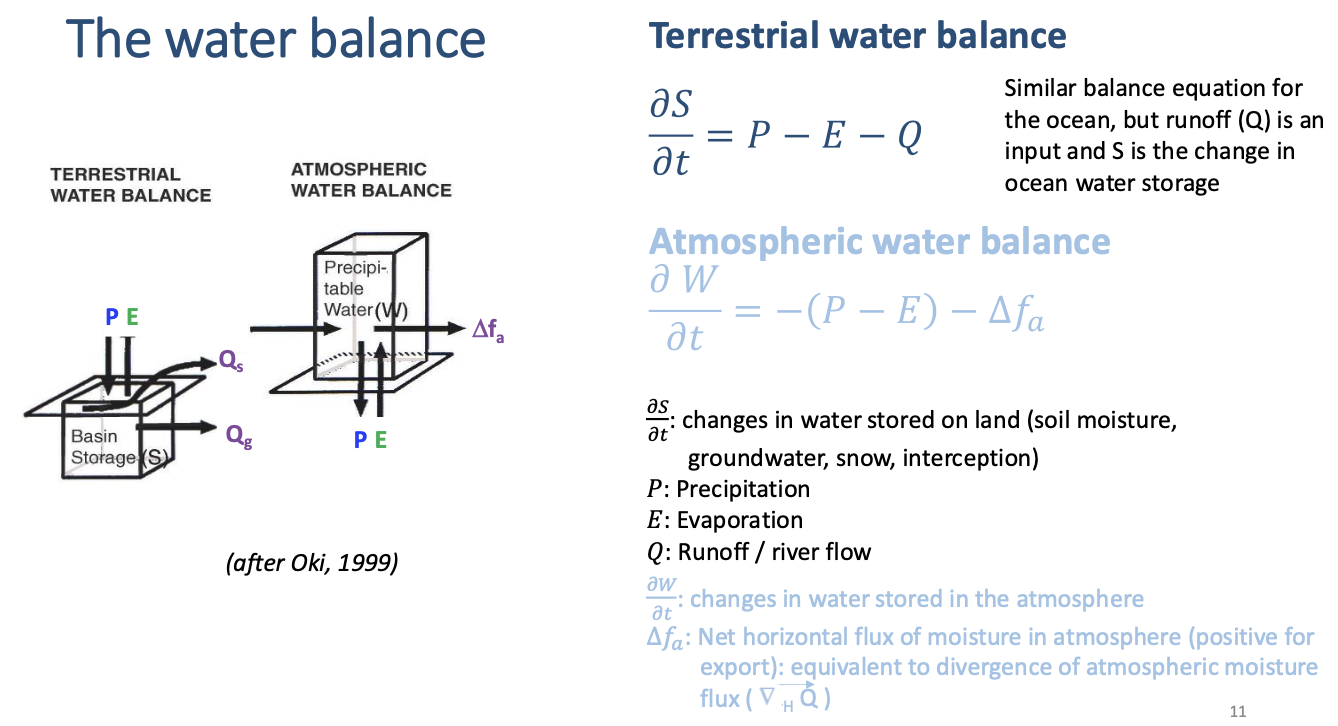
\includegraphics[width=1\linewidth]{CS/img/Water_balance.png}
\end{figure}

\subsection{What Fuels the Global Hydrological Cycle?}
The hydrological cycle is ultimately driven by solar radiation, which powers evaporation. Incoming shortwave radiation heats the surface, enabling water to evaporate. The latent heat required for evaporation is drawn from the surface energy budget. This cycle is thus fundamentally tied to Earth's energy balance.

\subsection{Energy and Water Coupling}
\begin{itemize}
    \item The surface energy balance is expressed as:
    \[
    R_s = \lambda E + SH + G + \Delta F_{eo}
    \]
    where:
    \begin{itemize}
        \item $R_s$: Net radiative energy at the surface
        \item $\lambda E$: Latent heat flux (evaporation/condensation)
        \item $SH$: Sensible heat flux
        \item $G$: Ground heat flux
        \item $\Delta F_{eo}$: Horizontal subsurface energy flux
    \end{itemize}
    \item The latent heat flux is directly linked to evaporation:
    \[
    E = \frac{LE}{\lambda}, \quad \text{where } \lambda = 2.5 \times 10^6 \, \text{J/kg}
    \]
    \item More net radiation $\Rightarrow$ more energy available for $\lambda E$ $\Rightarrow$ more evaporation $\Rightarrow$ more water vapor in the atmosphere $\Rightarrow$ more precipitation.
    \item Thus, the energy balance and water cycle are tightly coupled and co-regulate surface climate.
\end{itemize}

\subsection{Water in the Atmosphere}
\begin{itemize}
    \item Key quantities:
    \begin{itemize}
        \item \textbf{Vapor pressure ($e$):} Partial pressure of water vapor.
        \item \textbf{Specific humidity ($q$):} Mass of vapor per mass of air.
        \item \textbf{Mixing ratio ($r$):} Mass of vapor per mass of dry air.
    \end{itemize}
    \item Water vapor concentration decreases rapidly with altitude—most moisture is in the lower troposphere.
    \item The \textbf{Clausius-Clapeyron relation} describes the exponential increase in saturation vapor pressure with temperature ($\alpha_\nu$ specific volume of water vapor, $\alpha_l$ specific volume of liquid water):
    \[
    \frac{de_s}{dT} = \frac{\lambda }{ T(\alpha_\nu -\alpha_l)}
    \Rightarrow e_s(T) \approx 6.11 \cdot \exp\left[\frac{\lambda}{R_v} \left(\frac{1}{273} - \frac{1}{T}\right)\right]
    \]
    \item Warmer air can hold more moisture → amplified evaporation and precipitation in a warmer climate.
\end{itemize}

\subsection{Evapotranspiration}

Evapotranspiration is the sum of water loss from the Earth's surface through both evaporation and plant transpiration, linking the water and energy cycles.

\begin{itemize}
    \item \textbf{Evapotranspiration ($E$)} = evaporation + plant transpiration.
    \item It is driven by surface energy availability and modulated by:
    \begin{itemize}
        \item \textbf{Water holding capacity of air}, governed by temperature.
        \item \textbf{Availability of water at the surface}, much higher over oceans than land.
        \item \textbf{Vegetation properties}, which regulate transpiration via stomatal control.
    \end{itemize}
    
    \item \textbf{Energy balance and latent heat flux:}
    \begin{itemize}
        \item The latent heat flux ($\lambda E$) represents the energy used for evapotranspiration.
        \item It can be approximated as:
        \[
        \lambda E = R_s - \text{SH} - \Delta F_{eo} - G
        \]
        where:
        \begin{itemize}
            \item $R_s$: Net shortwave radiation
            \item SH: Sensible heat flux
            \item $\Delta F_{eo}$: Change in outgoing longwave radiation
            \item $G$: Ground heat flux
        \end{itemize}
        \item $\lambda E$ is both an energy and water flux, fundamental for linking the surface energy budget with the hydrological cycle.
    \end{itemize}

    \item \textbf{Spatial patterns of $\lambda E$:}
    \begin{itemize}
        \item \textbf{Largest values:} over warm mid-latitude ocean currents (e.g. Gulf Stream), and subtropical oceans.
        \begin{itemize}
            \item Here, evaporation consumes most of the energy provided by net radiation.
            \item This process drives atmospheric circulation and the hydrological cycle.
        \end{itemize}
        \item \textbf{Smallest values:} over land, especially in arid regions.
        \begin{itemize}
            \item Here, evaporation is limited by water availability.
        \end{itemize}
    \end{itemize}

    \item Overall, evapotranspiration plays a crucial role in shaping both weather and climate through its impact on the energy and water cycles.
\end{itemize}

\subsection{Precipitation Formation and Patterns}
\begin{itemize}
    \item \textbf{Three steps to precipitation:}
    \begin{enumerate}
        \item Supersaturation of air parcel - usually from adiabatic cooling during uplift.
        \item Droplet/ice formation around condensation nuclei.
        \item Droplet growth by collision/coalescence or aggregation until terminal velocity is reached.
    \end{enumerate}
    \item \textbf{Global patterns:}
    \begin{itemize}
        \item Highest precipitation in the ITCZ ( Inter Tropical Convergence Zone) and over tropical oceans.
        \item Lowest values in subtropical deserts and continental interiors.
    \end{itemize}
\end{itemize}

\subsection{Water Balance Across Regions}
\begin{itemize}
    \item Long-term atmospheric water storage is approximately constant:
    \[
    \frac{\Delta W}{\Delta t} \approx 0 \Rightarrow \Delta f_a = E - P
    \]
    \item \textbf{Regional contrasts:}
    \begin{itemize}
        \item Over oceans: $E > P$ → net export of moisture.
        \item Over land: $P > E$ → net import of moisture from oceans.
    \end{itemize}
    \item Runoff ($Q$) occurs when precipitation exceeds evaporation and storage change:
    \[
    Q = P - E - \frac{dS}{dt}
    \]
    \item Storage ($S$) includes soil moisture, groundwater, snowpack, etc.
\end{itemize}

\subsection{Streamflow and River Discharge}
\begin{itemize}
    \item Runoff accumulates to form streamflow and river discharge.
    \item \textbf{River discharge} = lateral transport of freshwater from land to oceans.
    \item Flow patterns depend on:
    \begin{itemize}
        \item Precipitation regime (e.g., monsoons, snowmelt)
        \item Topography (basin shape and elevation)
        \item Human factors (land use, dams, irrigation)
    \end{itemize}
    \item Good indicator of renewable water availability.
\end{itemize}

\subsection{Climate Change and the Water Cycle}
\begin{itemize}
    \item \textbf{Physical feedbacks:}
    \begin{itemize}
        \item Higher temperatures → higher vapor pressure → intensified evaporation and precipitation extremes.
        \item Water vapor enhances the greenhouse effect → further warming.
    \end{itemize}
    \item \textbf{Observed changes (IPCC AR6):}
    \begin{itemize}
        \item "When it rains, it pours": increased heavy precipitation events.
        \item Simultaneously, more drying of soils and longer dry spells.
        \item Switzerland: Fewer wet years, more dry years, declining snowpack.
    \end{itemize}
    \item \textbf{Projected trends:}
    \begin{itemize}
        \item Global mean $P$ and $E$ increase with warming.
        \item Subtropical drying and high-latitude moistening.
        \item Greater seasonality and variability in water availability.
        \item Dry-season runoff declines due to stronger evapotranspiration.
    \end{itemize}
\end{itemize}

\section{Terrestrial Biomes and Land-Climate Processes}
\noindent \textcolor{orange}{
Goal: Understand the role of land surfaces in the climate system. Flow: Starts from climate feedbacks across timescales, moves into land energy/water/carbon balances, feedbacks like soil moisture-temperature, human land use, and finally monitoring/observation systems.
}

\begin{figure}[H]
    \centering
    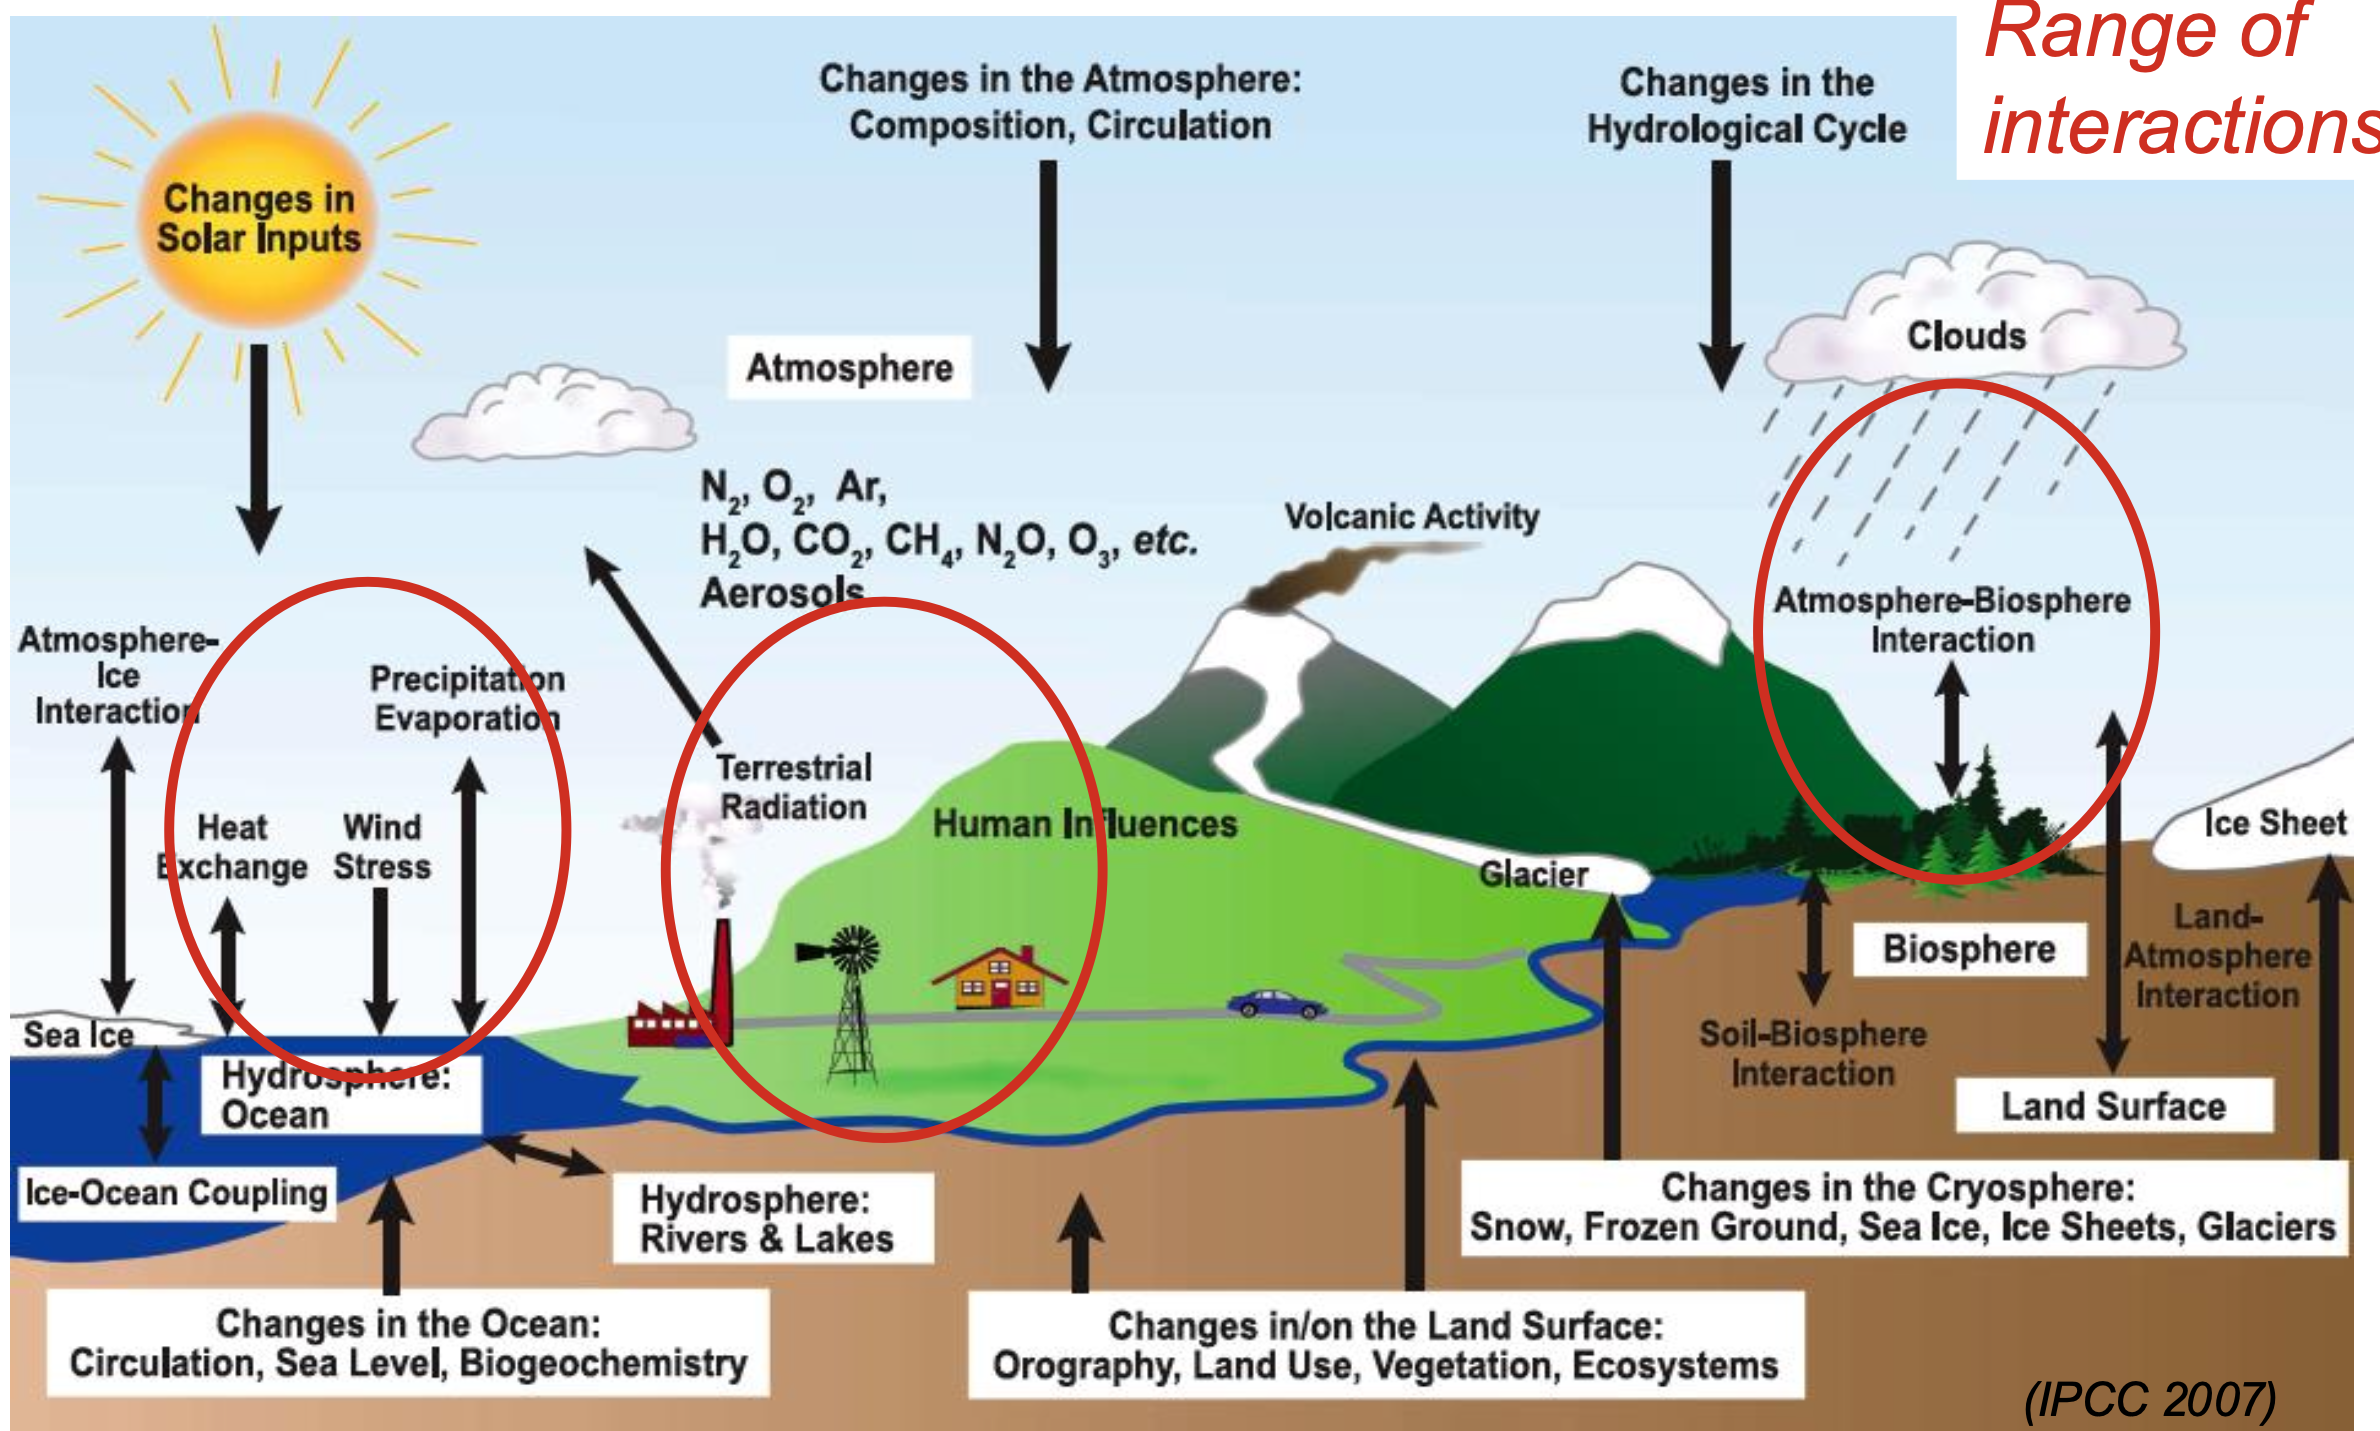
\includegraphics[width=\linewidth]{CS/img/Terrestrial Biomes, Land-climate processes.png}
\end{figure}
\subsection{Feedbacks in the Land-Climate System}
\begin{itemize}
    \item \textbf{Minutes–Hours:} Turbulent energy/moisture exchange (e.g., evapotranspiration).
    \item \textbf{Days–Weeks:} Ecosystem physiology and phenology, infiltration, runoff.
    \item \textbf{Years–Centuries:} Vegetation dynamics, carbon storage changes.
\end{itemize}
\begin{figure}[H]
    \centering
    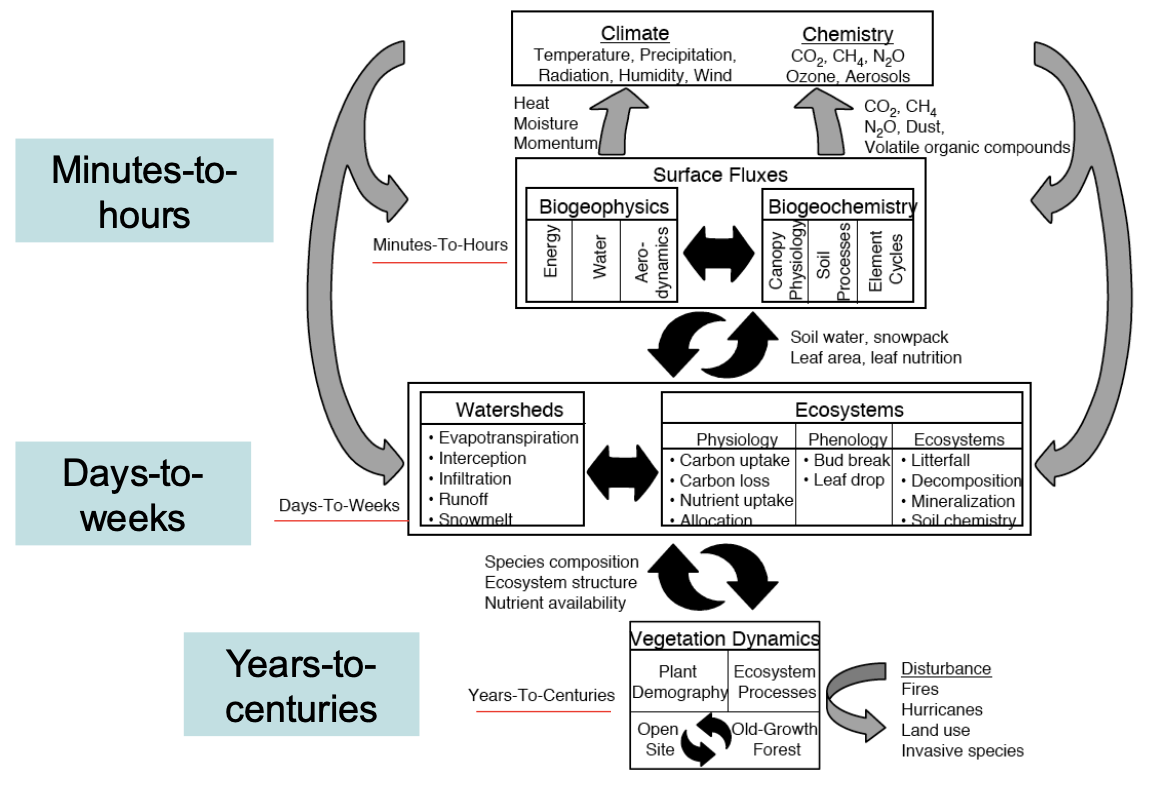
\includegraphics[width=\linewidth]{CS/img/Land_Climate_across_timescales.png}
\end{figure}

\subsection{Land Processes in the Climate System}
\noindent \textcolor{orange}{Slides 6–9: Land plays a central role in regulating climate via coupled water, energy, and carbon exchanges.}

\begin{itemize}
    \item The land surface is not a passive boundary — it actively controls exchanges of:
    \begin{itemize}
        \item \textbf{Water:} through evaporation, transpiration, infiltration, and runoff. About \textbf{60\% of precipitation} over land is recycled back into the atmosphere via evapotranspiration.
        \item \textbf{Energy:} via radiation absorption, heat flux partitioning (latent vs. sensible), and surface roughness effects. Approximately \textbf{50–60\% of net radiation} at the land surface is used for evapotranspiration (latent heat).
        \item \textbf{Carbon:} through photosynthesis, respiration, and decomposition. Terrestrial ecosystems currently absorb about \textbf{25–30\% of anthropogenic CO$_2$ emissions}.
    \end{itemize}
\end{itemize}

\begin{figure}[H]
    \centering
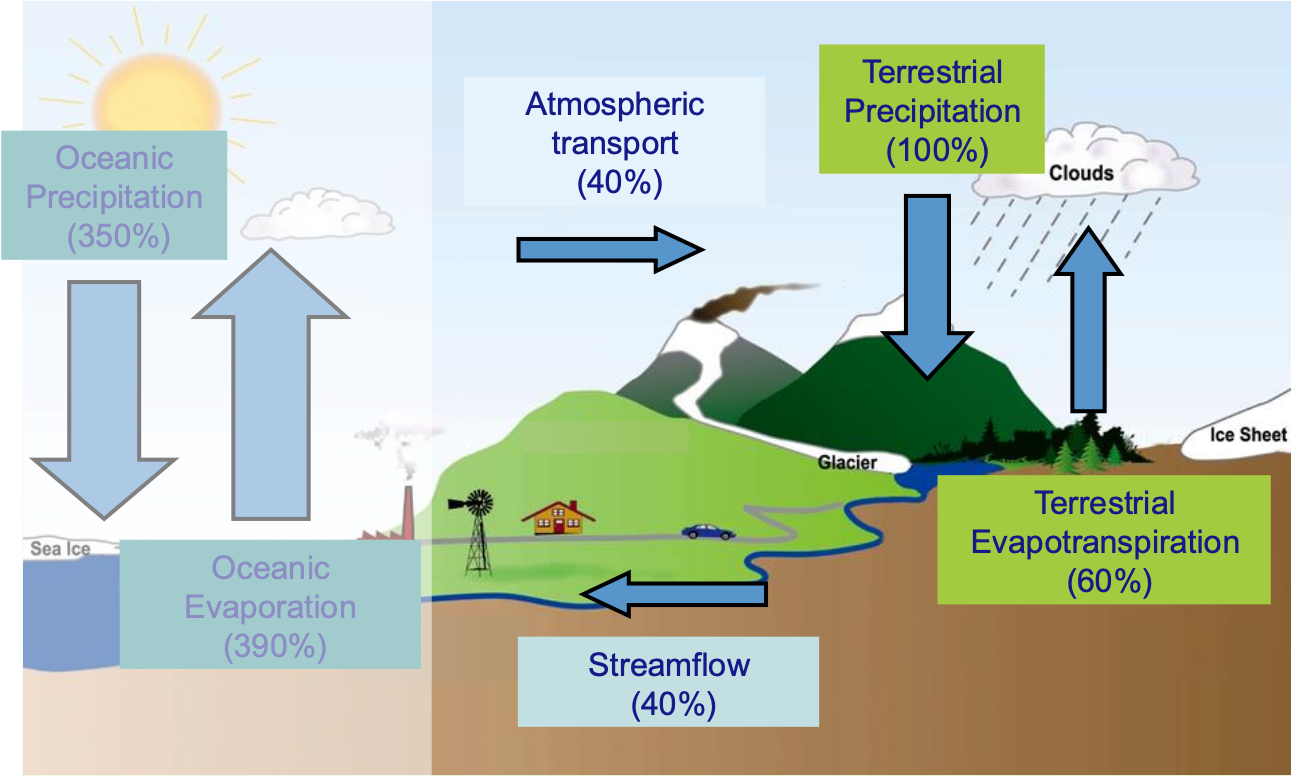
\includegraphics[width=1\linewidth]{CS/img/global_water_cycle.png}
\end{figure}

\textbf{Importance of vegetation:} E = soil evaporation + interception + transpiration, Half of the water flux to the atmosphere is conveyed by plants thus Biological processes play a major role in controlling evapotranspiration\\
Human activities have  modified the global
distribution of vegetation $\rightarrow$Anthropogenic forcing with consequences on climate 
\begin{figure}[H]
    \centering
    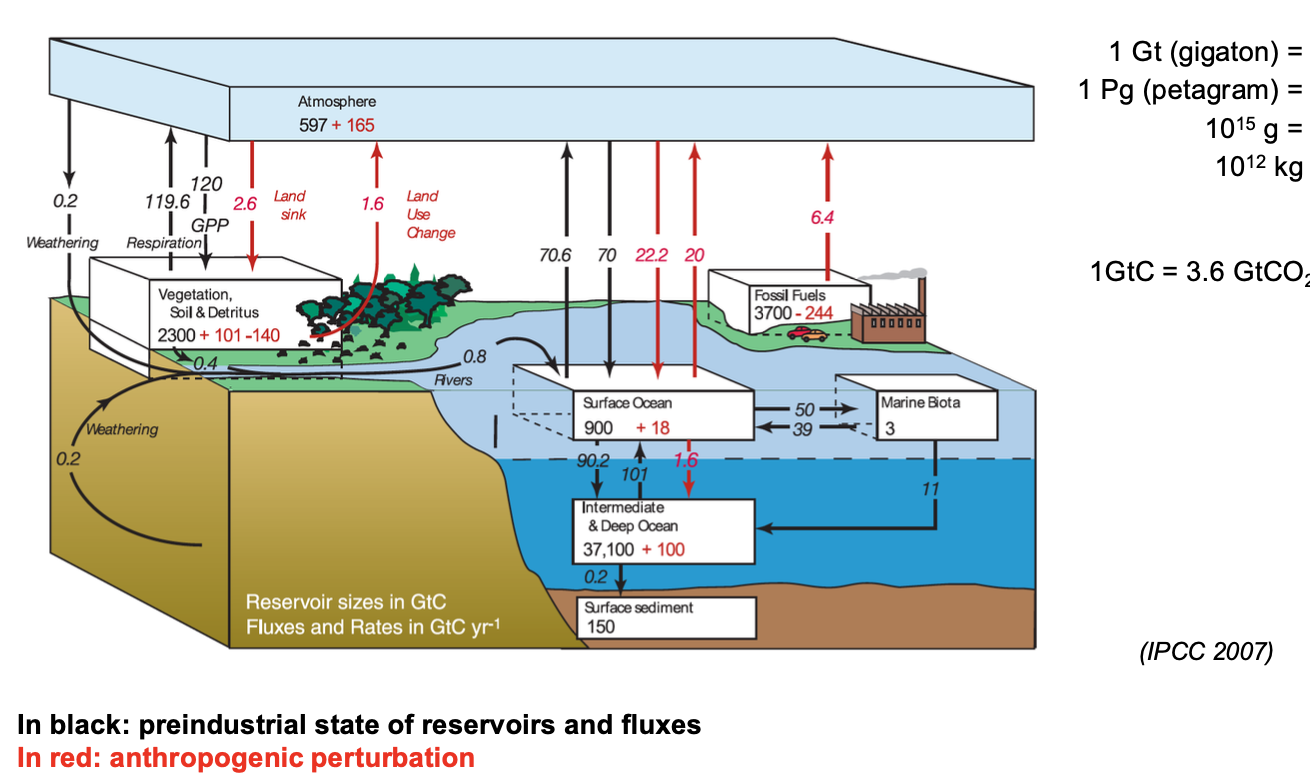
\includegraphics[width=1\linewidth]{CS/img/Global_C02_cycle.png}
\end{figure}

\subsection{Land energy, water, and carbon balances}
\noindent \textcolor{orange}{Slides 18–21: Coupled equations linking net radiation, latent heat, and runoff.}

\begin{figure}[H]
    \centering
    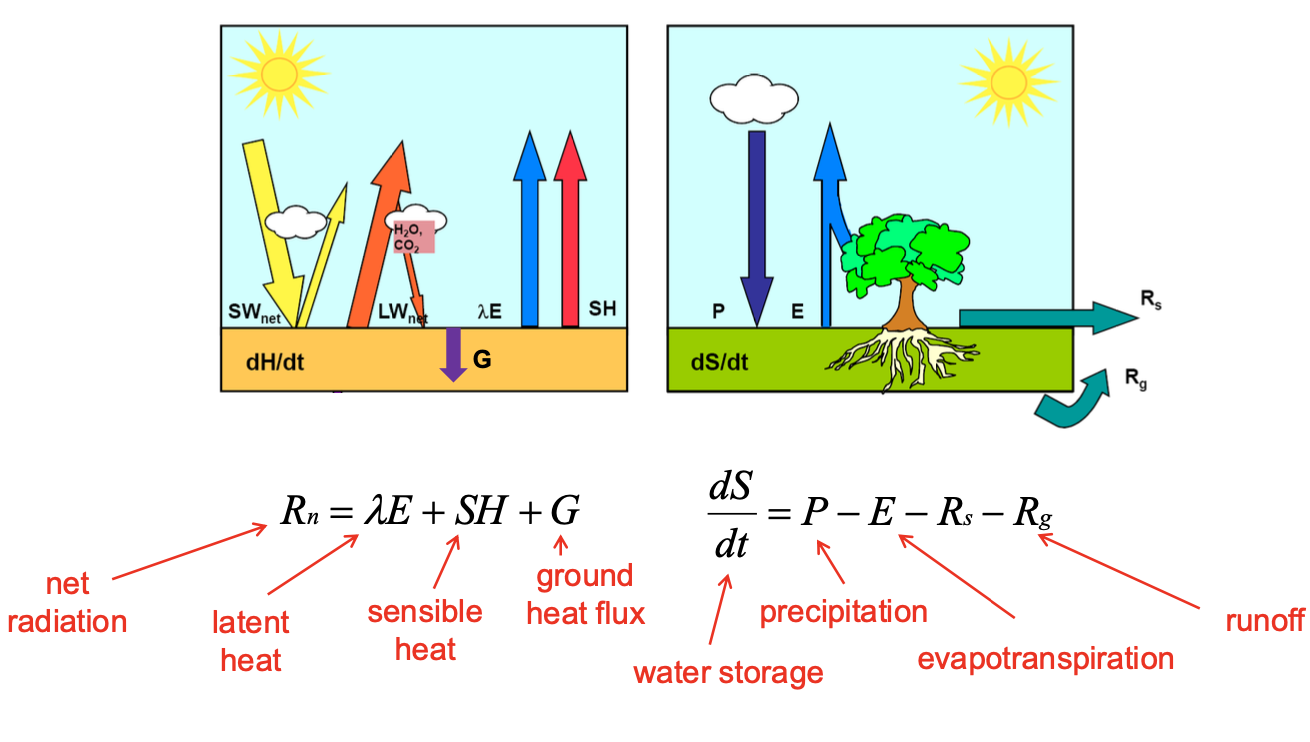
\includegraphics[width=1\linewidth]{CS/img/Energy_water_balance.png}
\end{figure}

\begin{itemize}
    \item $R_n$ is the NET radiation, so $R_n = \text{incoming solar radiation} - \text{reflected solar radiation} - \text{outgoing longwave radiation}$
    \item \textbf{Evapotranspiration (ET)} is a key process coupling the \textbf{energy and water balances} of the land surface.
    \item It transfers water from land to atmosphere and simultaneously removes energy via \textbf{latent heat flux} ($\lambda = 2454$ J/g for liquid water 20 degrees to water vapor, $\lambda = 4.2$ J/g for liquid water at 20 to 21 degrees and $\lambda = 1$ J/g for air at 20 to 21 degrees).
    \item \textbf{Roughly 50–60\% of net radiation} is used to drive ET, highlighting its role as a major energy sink.
    \item The \textbf{partitioning of surface energy} (latent vs. sensible heat) depends on vegetation cover, soil moisture, and land type.
    \item Therefore, changes in ET influence both surface temperature and atmospheric moisture, making it central to land–atmosphere interactions.
\end{itemize}
\subsection{Measurement of Turbulent Fluxes}
\noindent \textcolor{orange}{Slides 22–31: Measuring land–atmosphere exchanges of energy, water, CO$_2$, and momentum using eddy-covariance and the Bowen ratio.}

\begin{itemize}
    \item \textbf{Goal:} Quantify vertical exchanges of momentum, heat, moisture, and CO$_2$ between land surface and atmosphere, driven by turbulence.

    \item \textbf{Mathematical Foundation – Reynolds Decomposition:}
    \begin{itemize}
        \item Atmospheric quantities are separated into a mean and a fluctuating component:
        \[
        \phi(t) = \overline{\phi} + \phi'(t)
        \]
        \item Vertical turbulent fluxes are expressed as:
        \[
        \text{Flux} = \overline{w' \phi'}
        \]
        \item This covariance quantifies net vertical transport by eddies across a horizontal plane.
    \end{itemize}

    \item \textbf{Eddy-Covariance Technique:}
    \begin{itemize}
        \item Measures high-frequency (10–20 Hz) fluctuations in:
        \begin{itemize}
            \item \( u \): horizontal wind (momentum anomaly)
            \item \( w \): vertical wind (transports scalars vertically)
            \item \( T \): air temperature (sensible heat anomaly)
            \item \( q \): specific humidity (moisture anomaly)
            \item \( c \): CO$_2$ concentration (carbon anomaly)
        \end{itemize}
        \item These are used to compute turbulent fluxes:
        \begin{itemize}
            \item \textbf{Momentum (shear stress):} \( \tau = \rho \overline{u'w'} \)  
            Positive when wind momentum is transferred toward the surface.
            \item \textbf{Sensible heat:} \( H = \rho c_p \overline{w'T'} \)  
            Positive when heat is transported from the surface upward.
            \item \textbf{Latent heat:} \( \lambda E = L_v E = \rho \lambda \overline{w'q'} \)  
            Positive when moisture is evaporated and transported upward (i.e. evapotranspiration).
            \item \textbf{CO$_2$ flux:} \( F_{\text{CO}_2} = \overline{w'c'} \)
        \end{itemize}
        \item \textbf{Latent heat flux via eddies:} When $w'$ and $q'$ have the same sign, moist air rises (or dry air sinks) → net upward evapotranspiration flux.
        \item \textbf{Surface consistency:} In homogeneous terrain, boundary-layer moisture flux $\approx$ surface ET, though advection may still play a role.
    \end{itemize}
    \begin{itemize}
    \item \textbf{Alternatively turbulent fluxes can be considered in the same way as molecular fluxes} to obtain diffusion-like equations: $K_M$ (eddy turbulent viscosity) and $K_H$ and $K_E$ are eddy diffusivities. All are exchange coefficients (in m$^2$/s)
    \[
    \tau = -\rho \overline{w'u'} = \rho K_M \frac{\partial U}{\partial z}
    \]
    \[
    H = -\rho c_p \overline{w'T'} = -\rho c_p K_H \frac{\partial \theta}{\partial z}
    \]
    \[
    L_v E = -\rho L_v \overline{w'q'} = -\rho L_v K_E \frac{\partial Q}{\partial z}
    \]

    \item \textbf{Further alternative description: electrical current analogy} aerodynamic resistances $r_{aM}$, $r_{aH}$, $r_{aE}$ are the aerodynamic resistances for momentum, sensible heat and evaporative heat respectively. However surface value definition not always that simple. Resistances can be put in series or parallel depending on format of transport
    \[
    \tau = -\rho \overline{w'u'} = \rho K_M \frac{U - U_0}{r_{aM}}
    \]
    \[
    H = -\rho c_p \overline{w'T'} = -\rho c_p \frac{\theta - \theta_0}{r_{aH}}
    \]
    \[
    L_v E = -\rho L_v \overline{w'q'} = -\rho L_v \frac{Q - Q_0}{r_{aE}}
    \]
\end{itemize}
\item \textbf{The Bowen Ratio}
\begin{itemize}
    \item Concept used in meteorology and environmental science to describe the relationship between the sensible heat flux and the latent heat flux at the Earth's surface.
    \item It is defined as:
    \[
    \text{Bowen Ratio} = \frac{H}{L_v E}
    \]
    \item Inspired by the fact that experimental evidence indicates that aerodynamic transfer of heat and moisture through turbulence takes place in complete analogy.
    \item In general, we assume:
    \begin{itemize}
        \item \textbf{Higher Bowen ratio:} Drier surface conditions.
        \item \textbf{Lower Bowen ratio:} Wetter surface conditions.
    \end{itemize}
    \item Quantifies the moisture state at the surface.
    \item Indicates surface wetness and energy partitioning:
    \begin{itemize}
        \item \textbf{Low (e.g. 0.2):} Moist surface, more energy goes into evaporation.
        \item \textbf{High (e.g. more than 1):} Dry surface, more energy heats the air.
    \end{itemize}
\end{itemize}
\end{itemize}

\subsection{Land Carbon Balance}
\begin{itemize}
    \item \textbf{GPP (Gross Primary Production):} Total amount of carbon fixed by plants through photosynthesis. \\
    \textit{Global estimate:} $\sim$120 GtC yr$^{-1}$
    
    \item \textbf{NPP (Net Primary Production):} GPP minus autotrophic respiration (plant respiration). \\
    \textit{Global estimate:} $\sim$60 GtC yr$^{-1}$
    
    \item \textbf{NEE or NEP (Net Ecosystem Exchange/Production):} NPP minus heterotrophic respiration (e.g. soil microbes). \\
    \textit{Global estimate:} $\sim$10 GtC yr$^{-1}$
    
    \item \textbf{NBE or NBP (Net Biome Exchange/Production):} NEP/NEE minus losses from disturbances such as fires, deforestation, or soil tillage. \\
    \textit{Global estimate:} $\sim$+1 GtC yr$^{-1}$
\end{itemize}

\subsection{Coupling of Carbon and Water Balance by Plants and Stomata}
\noindent \textcolor{orange}{Slides 33–37: Stomatal control links plant transpiration and photosynthesis, coupling carbon, water, and energy fluxes.}

\begin{itemize}
    \item \textbf{Stomata} are microscopic pores in plant leaves that regulate gas exchange:
    \begin{itemize}
        \item Allow CO$_2$ to enter for photosynthesis (GPP).
        \item Release H$_2$O vapor through transpiration.
        \item Open/close depending on environmental conditions and plant species.
    \end{itemize}

    \item \textbf{Water-Use Efficiency:}
    \begin{itemize}
        \item Plants aim to maximize carbon gain per unit of water lost.
        \item Leads to trade-off: more CO$_2$ uptake $\rightarrow$ more water loss.
    \end{itemize}
    
    \item \textbf{Drought Response:}
    \begin{itemize}
        \item Under water stress, stomata close to reduce water loss.
        \item This reduces transpiration (latent heat flux) and CO$_2$ uptake (GPP).
        \item Strong impact on energy, water, and carbon balances.
    \end{itemize}

    \item \textbf{Implications for Climate Modeling:}
    \begin{itemize}
        \item Vegetation acts as a regulator of water and CO$_2$ fluxes.
        \item Climate models often \textit{underestimate} the sensitivity of CO$_2$ uptake to water availability.
    \end{itemize}

    \item \textbf{Core Coupling Concept:}
    \begin{itemize}
        \item Stomata couple the energy (via ET), water (via transpiration), and carbon (via GPP) cycles.
        \item These land-atmosphere exchanges of energy, water, and bio-geochemical fluxes are mediated by stomatal behavior.
    \end{itemize}

    \item \textbf{Key Quote:}
    \begin{quote}
    “Plants exert a strong control on the flow of water from the land masses into the atmosphere. They tend to maintain an optimal balance between limitation of H$_2$O loss and admission of CO$_2$, thus influencing the release and uptake of the two most important greenhouse gases.”
    \end{quote}
\end{itemize}
\begin{figure}[H]
    \centering
    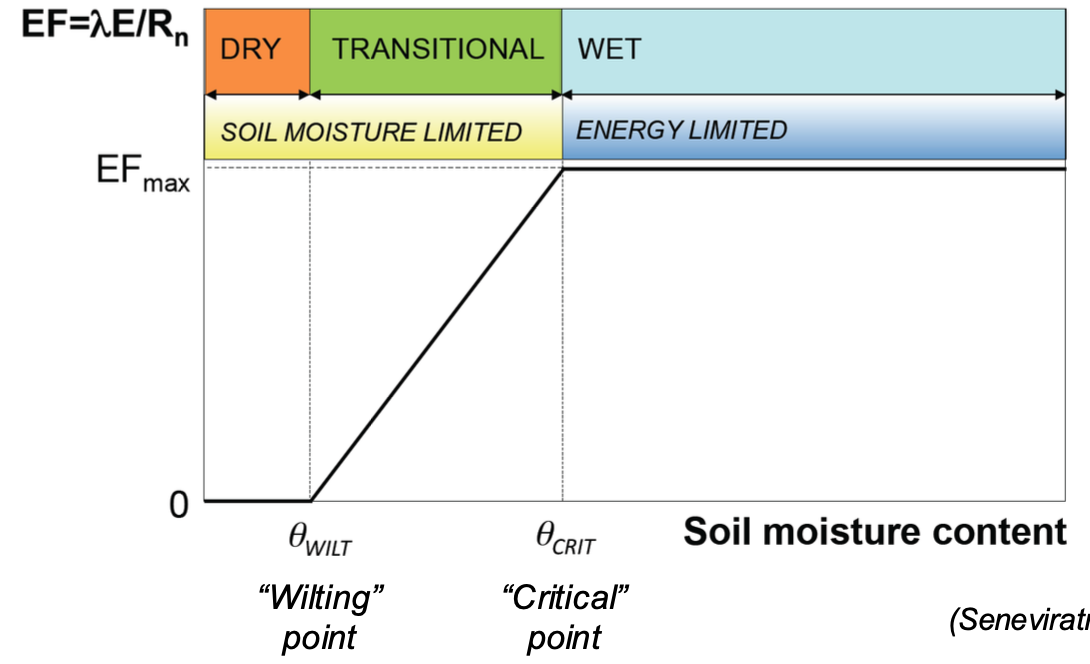
\includegraphics[width=1\linewidth]{CS//img/Schematic representation of soil moisture effects.png}
\end{figure}

\subsection{Soil Moisture–Temperature Feedback}
\noindent \textcolor{orange}{Slides 36–41: Dry soils reduce ET, increase H, and amplify temperature.}

\begin{itemize}
    \item \textbf{Evaporative cooling:} Land surface temperature is regulated by evapotranspiration — water evaporates and carries away energy as latent heat, reducing sensible heat and thus cooling the surface.
    
    \item \textbf{Low soil moisture:} When soil moisture is low:
    \begin{itemize}
        \item Less water is available for evapotranspiration.
        \item Cooling by evaporation becomes ineffective.
        \item More energy goes into sensible heat $\Rightarrow$ higher land surface temperature.
    \end{itemize}

    \item \textbf{Wilting point:} Critical soil moisture threshold at which plant transpiration and evaporation significantly drop, leading to abrupt surface warming.

    \item \textbf{Bowen Ratio Implication:}
    \begin{itemize}
        \item High Bowen ratio: lower latent heat, higher sensible heat $\Rightarrow$ dry surface.
        \item Low Bowen ratio: moist surface, more energy used for ET.
    \end{itemize}
    
    \item \textbf{Heatwave Amplification:} Drought and heatwaves are coupled:
    \begin{itemize}
        \item Dry soils enhance heat extremes.
        \item Feedback loop: drought $\rightarrow$ soil drying $\rightarrow$ reduced ET $\rightarrow$ warming $\rightarrow$ more drying.
    \end{itemize}

    \item \textbf{Modeling Note:} Many climate models do not initialize soil moisture realistically, underestimating the strength of land-atmosphere feedbacks.

    \item \textbf{Quantified Impact:} In hot-spot regions, soil moisture drying accounts for up to \textbf{30\% of projected regional warming}.

    \item \textbf{Irrigation Effects:} Irrigation increases soil moisture, enhancing ET and local cooling — until water becomes unavailable, at which point the feedback flips rapidly.
\end{itemize}

\subsection{Observational Evidence}
\noindent \textcolor{orange}{Slides 42–45: Empirical link between SPI (drought) and number of hot days.}

\begin{itemize}
    \item GLACE-CMIP5 shows soil moisture drying enhances warming projections.
    \item ~30\% of TXx (hottest day of year) increases tied to soil drying.
\end{itemize}

\subsection{Regional vs Global Warming}
\noindent \textcolor{orange}{Slide 47: Extremes warm more than global mean due to soil and albedo feedbacks.}

\begin{itemize}
    \item A global 1.5°C warming may imply >3°C warming in regional extremes.
\end{itemize}

\subsection{Droughts and Climate Change}
\noindent \textcolor{orange}{Slides 50–52: Drought risk increases with warming even if precipitation does not drop.}

\begin{itemize}
    \item \textbf{Evapotranspiration increases} with temperature, which can offset or outweigh any increase or stability in precipitation — leading to net \textbf{soil drying}.
    \item \textbf{Soil moisture declines} are more extensive than precipitation reductions because warming enhances evaporation.
    \item Many \textbf{“drying regions”} are experiencing more frequent and intense droughts due to increased ET under climate change.
    \item \textbf{IPCC AR6} confirms widespread intensification of droughts in subtropical and temperate regions.
\end{itemize}

\subsection{Land Use and Land Cover Change}
\noindent \textcolor{orange}{Slides 54–56: Combined biophysical and carbon effects vary by biome.}

\begin{itemize}
    \item \textbf{Biophysical effects} (e.g., albedo, ET capacity) and \textbf{biogeochemical effects} (e.g., CO$_2$ sinks) must be considered jointly.
    \item \textbf{Tropical forests} cool the climate mainly through strong carbon uptake.
    \item \textbf{Boreal forests} may cause regional warming due to their low albedo (dark surface absorbing more radiation).
    \item \textbf{Afforestation and BECCS (Bioenergy with CCS)}: Only effective for climate mitigation where cooling from CO$_2$ uptake outweighs warming from changes in albedo or ET.
    \item \textbf{Land management} practices — such as no-till farming, irrigation, and double cropping — influence water availability, albedo, and carbon fluxes.
    \item During \textbf{heatwaves}, forests have been observed to \textbf{evaporate less than grasslands}, leading to net surface warming. Forests are more conservative with water use, reversing expected cooling under drought.
    \item \textbf{Vegetation–climate feedback}: Climate impacts vegetation (e.g., via forest fires), but this is often not represented in Integrated Assessment Models (IAMs) — making them overly optimistic.
    \item \textbf{Soil moisture data} is scarce at global scale, limiting model validation and regional analysis.
    \item There is a growing need for \textbf{observational intercomparison projects} — not just model intercomparisons — to benchmark and improve understanding of land–climate processes.
    \item New developments include \textbf{ground networks}, \textbf{new satellite missions}, and \textbf{data merging projects}, which aim to close the observational gap.
\end{itemize}

\subsection{Evaporation in Forests vs Grasslands}
\noindent \textcolor{orange}{Slides 57–59: Under drought, forests may reduce ET more than grass.}
\begin{figure}[H]
    \centering
    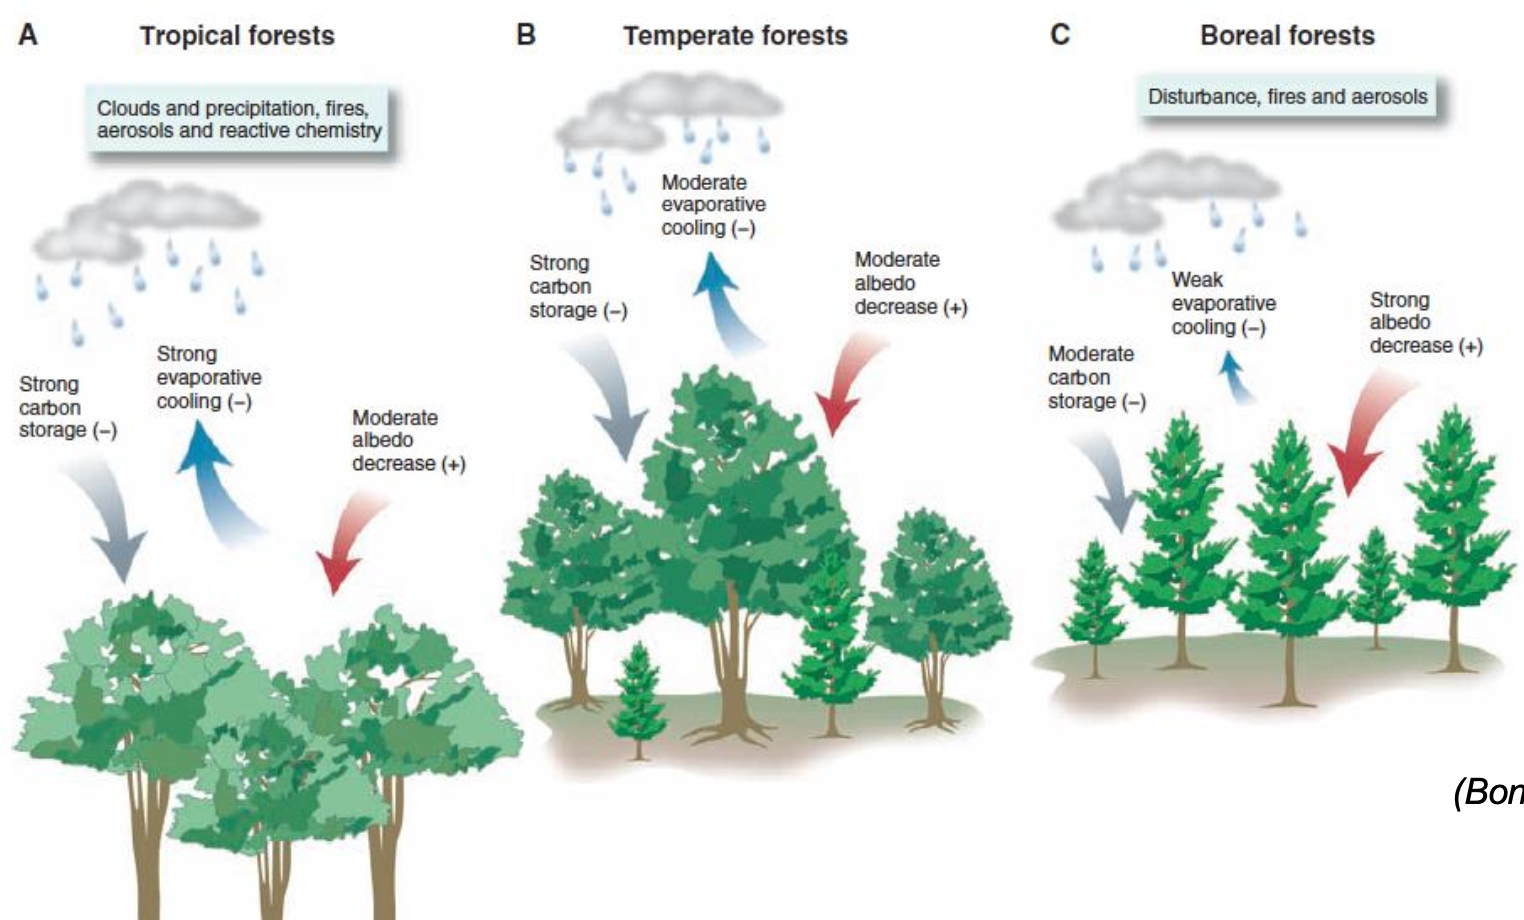
\includegraphics[width=1\linewidth]{CS//img/Forest_difference_effect_clima.png}
\end{figure}
\begin{itemize}
    \item Trees: deep roots, but during drought ET suppressed more than grass.
    \item Satellite data show stronger soil warming under forests in 2003 heatwave.
\end{itemize}

\subsection{Land Management Effects}
\noindent \textcolor{orange}{Slides 60–64: No-till, double cropping, irrigation modify surface energy and carbon balance.}

\begin{itemize}
    \item No-till farming increases albedo and cools surface extremes.
    \item Management can enhance CO$_2$ sinks, but may be overestimated in IAMs.
\end{itemize}

\subsection{Observational Systems}
\noindent \textcolor{orange}{Slides 66–71: Instruments and networks that monitor ET, CO$_2$, and land moisture.}

\begin{itemize}
    \item \textbf{Ground:} SwissSMEX, FLUXNET.
    \item \textbf{Satellite:} SMOS, GRACE, NDVI, land albedo.
    \item \textbf{Challenge:} Still limited data coverage and resolution.
\end{itemize}

\subsection{Conclusions}
\noindent \textcolor{orange}{Slide 73: Land is both affected by and influences climate change.}

\begin{itemize}
    \item Key link between water, energy, and carbon cycles.
    \item Relevant for variability, extremes, weather prediction.
    \item Critical research area needing models + better observations.
\end{itemize}

\section{Detection and Attribution of Observed Climate Change}
\noindent\textcolor{orange}{
Goal: Learn how scientists detect and attribute climate change to human activity using models and statistical methods\\
Flow: Historical foundations $\rightarrow$ D\&A framework $\rightarrow$ fingerprint methods $\rightarrow$ precipitation, hydrology, extremes Introduces $\rightarrow$ statistical EEA basics $\rightarrow$ detailed case studies $\rightarrow$ model needs $\rightarrow$ storyline approaches $\rightarrow$ best practices.
}
\subsection{Scientific Foundations}
\begin{itemize}
    \item \textbf{Joseph Fourier (1824):} Proposed that the atmosphere acts as an \textit{insulating blanket}, warming Earth.
    \item \textbf{Eunice Foote (1856):} Demonstrated that CO2 \textit{traps more heat} than air under sunlight.
    \item \textbf{John Tyndall (1859):} Identified \textit{infrared absorption} by CO2, CH4, and H2O.
    \item \textbf{Svante Arrhenius (1896):} Linked \textit{fossil fuel emissions to global warming}, described \textit{water vapor feedback}.
    \item \textbf{G.S. Callendar (1938):} Quantified \textit{CO2-induced warming} consistent with observed temperature rise.
    \item \textbf{Syukuro Manabe (1967):} Developed the first \textit{1D climate model with convection}, showing CO2 leads to warming.
\end{itemize}

\subsection{Early evidence in support of human influence on
the climate system}
\begin{itemize}
    \item Increasingly well understood absorption and emission properties of gases
    \item Progress in numerical atmospheric modeling demonstrate consistent effects
    \item Observational evidence pointing to rising CO2 and temperature
\end{itemize}

\subsection{Detection and Attribution (D\&A) Framework}
\begin{itemize}
    \item \textbf{Detection:} Demonstrate that observed changes deviate from natural internal variability.
    \item \textbf{Attribution:} Attribution of anthropogenic climate change requires a demonstration that the detected change are 1. consistent with simulated change driven by anthropogenic changes in the composition of the atmosphere and 2. inconsistent with alternative explanations.
    \item \textbf{Approach:} Combine observational trends and model simulations to extract climate signals from noise.
\end{itemize}

\subsection{Attribution of Global Warming}

\begin{itemize}
    \item \textbf{Goal:} Separate the signal of anthropogenic climate change from natural internal climate variability.
    
    \item \textbf{Fingerprinting Concept:}
    \begin{itemize}
        \item Climate models simulate distinct patterns of temperature change ("fingerprints") for different forcings (e.g., greenhouse gases, solar variability, aerosols).
        \item Ensemble averaging across many simulations suppresses internal variability and enhances the forced signal.
    \end{itemize}
    
    \item \textbf{Regression Approach:}
    \[
        \text{OBS} = \beta_\text{ANT} \cdot \text{ANT} + \beta_\text{NAT} \cdot \text{NAT} + \text{Variability}
    \]
    \begin{itemize}
        \item $\text{OBS}$: Observed climate trend (e.g., GMST)
        \item $\text{ANT}$: Simulated response to anthropogenic forcing
        \item $\text{NAT}$: Simulated response to natural forcing
        \item $\beta$: Scaling factors (regression coefficients)
    \end{itemize}
    
    \item \textbf{Interpretation of $\beta$ values:}
    \begin{itemize}
        \item $\beta \approx 1$: Model simulations agree with observations.
        \item $\beta \approx 0$: Simulated effect not found in observations.
        \item Confidence intervals assess statistical robustness of detection.
    \end{itemize}
    
    \item \textbf{Signal-to-Noise Optimization:}
    \begin{itemize}
        \item Aggregating data spatially and temporally enhances signal strength.
        \item Helps distinguish forced climate signals from chaotic internal variability.
    \end{itemize}
    
    \item \textbf{Model Comparisons:}
    \begin{itemize}
        \item Observations are compared to both historical simulations (with full forcing) and counterfactual simulations (natural only).
        \item Only models including anthropogenic forcing replicate observed trends.
    \end{itemize}
    
    \item \textbf{Conclusion:} Consistent attribution results across models and observations confirm that recent global warming is primarily due to human-induced greenhouse gas emissions.
\end{itemize}

\subsection{Beyond Mean Temperature}

\begin{itemize}
    \item \textbf{Motivation:} Climate change does not only affect global mean temperature — impacts also manifest regionally and in other variables like precipitation and extremes.
    
    \item \textbf{Zonal Precipitation Trends (1950–1999):}
    \begin{itemize}
        \item Observed zonal precipitation trends show significant latitudinal structure.
        \item Models with anthropogenic forcing reproduce these trends; natural-only simulations do not.
        \item Attribution confirmed using regression of simulated fingerprints (Zhang et al., 2007).
    \end{itemize}
    
    \item \textbf{Concurrent Hot and Wet Extremes:}
    \begin{itemize}
        \item Spatially concurrent extreme temperature and precipitation events are increasing.
        \item Trend in land area simultaneously affected by extremes is consistent with historical simulations including human forcing (Biess et al., 2024).
        \item Early industrial (pre-1900) simulations do not show the same trends.
    \end{itemize}

    \item \textbf{Hydrological Trends:}
    \begin{itemize}
        \item \textbf{River Flow:} Trends in global river discharge from 1971–2010 show regional signals.
        \item Only simulations with historical radiative forcing (HIST) reproduce observed flow trends 
        \item \textbf{Lake Ice Duration:} Decline in freeze duration attributed to human influence. Only models with historical forcing match reconstructions 
        \item \textbf{Permafrost Thawing:} In situ temperature observations show warming trends consistent with simulations including anthropogenic forcing 
    \end{itemize}
    
    \item \textbf{Conclusion:} Human influence is detectable not just in temperature, but also in zonal precipitation, extremes, and the terrestrial hydrological system. These results confirm that climate change affects a wide range of Earth system processes.
\end{itemize}

\subsection{Extreme Event Attribution (EEA) Basics}

\begin{itemize}
    \item \textbf{Goal:} Quantify how anthropogenic climate change has altered the probability and intensity of specific weather or climate extremes (e.g., heatwaves, droughts).

    \item \textbf{Approach:} Compare climate model simulations of:
    \begin{itemize}
        \item \textbf{Factual world:} All forcings (natural + anthropogenic).
        \item \textbf{Counterfactual world:} Natural forcings only (e.g., solar variability, volcanic eruptions).
    \end{itemize}
    These allow us to isolate the effect of greenhouse gases and land-use change.

    \item \textbf{Step 1 – Fit Probability Distributions:}
    \begin{itemize}
        \item Use observed or simulated climate data to fit statistical models.
        \item Most common choices:
        \begin{itemize}
            \item \textbf{Gaussian distributions} for moderately extreme events.
            \item \textbf{Generalized Extreme Value (GEV)} distributions for rare or annual/block maxima events.
        \end{itemize}
    \end{itemize}

    \item \textbf{Step 2 – Estimate Probability Shifts:}
    \begin{itemize}
        \item Compute probability of exceeding a given threshold (e.g., temperature or drought index) in both climates.
        \item Calculate:
        \begin{itemize}
            \item \textbf{Probability Ratio (PR)} = $P_\text{factual} / P_\text{counterfactual}$
            \item \textbf{Attribution Statement:} e.g., “Human influence made this event X times more likely.”
        \end{itemize}
    \end{itemize}

    \item \textbf{Shifting Gaussian:}
    \begin{itemize}
        \item The mean $\mu$ of the Gaussian changes with global mean temperature (GMT): $\mu = a + b \cdot \text{GMT}$.
        \item The standard deviation $\sigma$ is held constant.
        \item Suitable for events like spring temperatures (e.g., March 2024 heat).
    \end{itemize}

    \item \textbf{Scaling Gaussian:}
    \begin{itemize}
        \item Both $\mu$ and $\sigma$ depend on GMT (e.g., soil moisture in summer).
        \item Captures changing variability in addition to shifting mean.
    \end{itemize}

    \item \textbf{Generalized Extreme Value (GEV) Distribution:}
    \begin{itemize}
        \item Used to model the distribution of block maxima (e.g., annual maximum temperature or precipitation).
        \item Enables probabilistic statements for extremely rare events with limited data.
        \item Alternative: Generalized Pareto Distribution (GPD) for peaks-over-threshold events.
    \end{itemize}

    \item \textbf{Why We Use Models:}
    \begin{itemize}
        \item Observational records are too short to estimate probabilities of rare extremes.
        \item Statistical models allow extrapolation beyond what has been observed.
        \item Fitting a distribution enables robust quantification of change even when exceedances are zero in the counterfactual world.
    \end{itemize}
\end{itemize}

\subsection{Case Study: March 2024 Heat in Europe}
\begin{itemize}
    \item Event would occur \textbf{once in 300 years} under pre-industrial conditions (globally about 1.2 °C cooler than now).
    \item Now expected \textbf{every 5 years}—probability increased by a factor of 60.
    \item Intensity of equally probable events has
    increased $>3^{\circ}$C.
\end{itemize}

\subsection{Why can’t we just use observations? And why do we need statistical models?}

\begin{itemize}
    \item For moderately extreme events (e.g. $>3^{\circ}$C), we can count threshold exceedances in two time periods:
    \begin{itemize}
        \item “Counterfactual” period (e.g. 1950–1986, less warming)
        \item “Factual” period (e.g. 1987–2023, current climate)
    \end{itemize}
    \item Example: For a 3°C threshold:
    \begin{itemize}
        \item 7 exceedances in the earlier period, 19 in the later $\rightarrow$ probability ratio (PR) $\approx$ 2.7
    \end{itemize}
\end{itemize}

\subsection{Problem with Rare Events}
\begin{itemize}
    \item For more extreme thresholds (e.g. $>5^{\circ}$C), we often observe 0 exceedances in the counterfactual period.
    \item This leads to undefined or infinite probability ratios.
    \item Observational records are too short to reliably estimate probabilities of rare events.
\end{itemize}

\subsection{Why Statistical Models are Needed}
\begin{itemize}
    \item Statistical models allow us to fit a continuous distribution to the data.
    \item This enables:
    \begin{itemize}
        \item Estimating probabilities even when no exceedance were observed.
        \item Quantifying uncertainty ranges.
        \item Comparing full distributions from factual and counterfactual climates.
    \end{itemize}
    \item Most extreme event attribution studies use:
    \begin{itemize}
        \item Gaussian distributions (for moderately extreme events)
        \item Generalized Extreme Value (GEV) distributions (for rare, block-maxima events)
    \end{itemize}
\end{itemize}

\subsection{Examples of EEA Studies}

\begin{itemize}
    \item \textbf{February 2025 Drought in Europe:}
    \begin{itemize}
        \item Recorded as the driest February in West-Central Europe in over 30 years.
        \item Observations from E-OBS v30.0e show severe precipitation deficits.
        \item Attributed to climate change using ERA5 data and ClimateExplorer analysis.
        \item Drought conditions consistent with intensification expected under global warming.
    \end{itemize}

    \item \textbf{2022 Summer Drought in Europe (Schumacher et al., 2024):}
    \begin{itemize}
        \item A peer-reviewed attribution study combining observational records and GCM-based simulations.
        \item Found that human-induced climate change made the drought significantly more likely and severe.
        \item Methodology used conditional distributions and scaling Gaussians to link low soil moisture to global mean temperature.
        \item Synthesized results showed that the observed event intensity cannot be explained without anthropogenic influence.
    \end{itemize}

    \item \textbf{South Sudan Heatwave (March 2025):}
    \begin{itemize}
        \item 7-day mean peak temperature was 4°C higher than what would be expected in a pre-industrial climate.
        \item World Weather Attribution (WWA) analysis concluded the event is ~1000 times more likely due to human-induced climate change.
        \item Confidence interval for increased probability ranged from 55 to infinity (95\% CI).
        \item This example highlights the power of attribution science to communicate climate risk in vulnerable regions.
    \end{itemize}
\end{itemize}

\subsection{Storyline Approach to EEA}

\begin{itemize}
    \item \textbf{Concept:}  
    A conditional attribution method focusing on how climate change influences the physical processes of a specific event, assuming a fixed large-scale atmospheric circulation.

    \item \textbf{Motivation:}  
    Useful when the signal-to-noise ratio is low, or probabilistic methods yield inconclusive results (e.g., rare circulation patterns, strong internal variability).

    \item \textbf{Key Features:}
    \begin{itemize}
        \item Does not compare event probabilities globally across many events.
        \item Conditions the analysis on the observed circulation pattern (e.g. blocking high, jet shift).
        \item Avoids false negatives ("Type II errors") common in probabilistic approaches.
    \end{itemize}

    \item \textbf{ClimaMeter Tool:}
    \begin{itemize}
        \item Searches for analogs of the observed atmospheric circulation (e.g., sea level pressure fields) in both factual and counterfactual time periods.
        \item Compares climate variables (e.g. temperature, humidity, fire risk) conditional on that circulation.
        \item Allows for fast attribution of regional events, e.g., wildfires or heatwaves.
    \end{itemize}

    \item \textbf{Example – March 2025 Wildfires in Korea and Japan:}
    \begin{itemize}
        \item Circulation pattern matched with historical analogs using ClimaMeter.
        \item Found that human-induced warming significantly amplified the fire risk under the given meteorological setup.
        \item Demonstrates how storyline attribution can highlight specific causal pathways.
    \end{itemize}

    \item \textbf{Trade-off:}
    \begin{itemize}
        \item While less general than probabilistic methods, storyline are often more physically interpretable and relevant for communication and decision-making.
    \end{itemize}
\end{itemize}

\subsection{Key EEA Principles}
\begin{itemize}
    \item Clear event definition and motivation for statistical model choice.
    \item Use multiple observational datasets and validated models.
    \item Report full uncertainty range (e.g., 95\% confidence intervals).
    \item Combine observational and modeling evidence to formulate attribution statements.
\end{itemize}


\end{multicols*}
\end{document}